\documentclass[solutions]{esg8022pset} 
\usepackage{amsmath}
\usepackage{amssymb}
\usepackage{enumerate}
\usepackage{graphicx}
\usepackage{hyperref}
\usepackage{mathtools}
\usepackage[per-mode=symbol]{siunitx} %If this line is giving you trouble, try replacing per-mode with per
%use inter-unit-separator={}\cdot{} ?
\providecommand{\uvec}[1]{{\hat{\bf{#1}}}}
\usepackage{pgf,tikz}
\usetikzlibrary{arrows}
\usepackage{wasysym}
\usepackage{subfig}
\makeatletter
\newcommand{\interitemtext}[1]{%
  \begin{list}{}
   {\itemindent=0mm\labelsep=0mm
   \labelwidth=0mm\leftmargin=0mm
   \addtolength{\leftmargin}{-\@totalleftmargin}}
    \item #1
  \end{list}
}
\makeatother
\renewcommand{\d}{\,d}
\providecommand{\norm}[1]{\lVert#1\rVert}

\newcommand{\Kgrad}{\left(\hat{x} \frac{\partial}{\partial x} + \hat{y} \frac{\partial}{\partial y} + \hat{z} \frac{\partial}{\partial z}\right)}
\newcommand{\Kdiv}[6]{{#4}\left(\frac{\partial {#1}}{\partial x} {#5} \frac{\partial {#2}}{\partial y} {#6}\frac{\partial #3}{\partial z} \right)}
\newcommand{\KKdiv}[6]{{#4}\left(\frac{\partial}{\partial x}{#1} {#5} \frac{\partial}{\partial y}{#2} {#6}\frac{\partial}{\partial z}{#3} \right)}
\newcommand{\dx}{\frac{\partial}{\partial x}}
\newcommand{\dy}{\frac{\partial}{\partial y}}
\newcommand{\dz}{\frac{\partial}{\partial z}}
\newcommand{\dtheta}{\frac{\partial}{\partial \theta}}
\newcommand{\dr}{\frac{\partial}{\partial r}}

\AtBeginDocument{%
  % Apologies to any future editor on the inconsistencies in TeX code and the unnecessary braces.  I'm aggregating previously typeset problems, and didn't think it worth my time to improve the quality of TeX code in ways that won't make any difference to the typeset material. -Jason Gross (jgross@mit.edu)
}%
\classname{Physics 8.022} \semester{Spring 2011} 
\problemsetnumber{10}
\date{\today }
\duedate{Wednesday, May 4th 10 am IN CLASS}
\readingassignment{}
\problemsettitle{Maxwell's equations, waves}
\begin{document}
\section{Problem \thesection: Discovery of magnetic charge}
\subsection{Problem}
You discover magnetic
charge.  The units of magnetic charge density,
$\mu$, are chosen such that $\vec\nabla\cdot\vec B = 4\pi\mu$.

\par\noindent (a) When this magnetic charge is in motion,
there is a ``magnetic current density'' $\vec {L} = \mu \vec{ v}$.  In
analogy to electric charge density and electric current densities,
write down the equation of continuity for magnetic charge.

\par\noindent (b) What do Maxwell's equations become with this
new charge? Hint: this vector identity may be useful.. $\vec\nabla\cdot(\vec{\nabla}\times\vec{F})=0$ for any $\vec{F}$.
\subsection{Solution}
(a) \begin{equation}
\frac{\partial \mu}{\partial t}+\vec{\nabla}\cdot\vec{L}=0.
\end{equation}
(b) Take the divergence of the $\vec\nabla\times\vec E$ equation; you'll
find that the new equation of magnetic charge continuity is violated.
To fix it, you must add a term that is proportional to $\vec L$ to
Faraday's law.  The resulting Maxwell equations are:

\begin{eqnarray}
\vec{\nabla}\times\vec{E} &=& -\frac{1}{c}\frac{\partial
\vec{B}}{\partial t}-\frac{4\pi}{c}\vec{L}\\
\vec{\nabla}\times\vec{B} &=& \frac{1}{c}\frac{\partial
\vec{E}}{\partial t}+\frac{4\pi}{c}\vec{J}\\
\vec{\nabla}\cdot\vec{E} &=& 4\pi\rho\\
\vec{\nabla}\cdot\vec{B} &=& 4\pi\mu.
\end{eqnarray}




\section{Problem \thesection:  Magnetic field of a moving charge}
\subsection{Problem}
A charge $q$ moving
along the $x$-axis at constant speed $v \ll c$.  When it is at $x =
-d$, what is the magnetic field at $(x,y,z) = (0,r,0)$?

\par\noindent (a)  Solve this first using Biot-Savart.  (Hint:
the current from the moving charge isn't particularly well defined.
However, B-S only needs the combination $I dl = (dq/dt) dl = dq
(dl/dt) \simeq q_{\rm pt\ charge}(dl/dt)$.  Sloppy physicist calculus
in action!)

\par\noindent (b)  Now solve this using displacement current.
Look at a circle of radius $r$ centered at the origin and passing
through the point $(0,r,0)$.  By symmetry, $\vec B$ will be constant
on this circle and oriented in the tangential direction.  Find a
surface which has this circle as a boundary and for which $\int \vec
E\cdot d\vec a$ is simple.  Evaluate this flux, apply the
``generalized'' form of Ampere's law (integral formulation) and you're
there.

\par\noindent Note, there's a third way: Lorentz transform from the
rest frame electric field.  All
three answers should agree, at least in the limit $v \ll c$.

\subsection{Solution}
a) Solve this first using Biot-Savart.\\

For low speed $v\ll c$, we can ignore the relativistic effects.  To
apply B-S law, we simply treat the moving charge at $x=-d$ as an
element current at the same location and $I d\vec{l}=qv\hat{x}$.  Then
we have
\begin{equation}
\vec{B}= \frac{qv\hat{x}\times\hat{r}_1}{cr_1^2},
\end{equation}
where $\vec{r}_1$ is the position vector from the moving charge to the
test point $(0,r,0)$.  Using $r_1 = \sqrt{r^2 + d^2}$ and $\hat
x\times\hat r_1 = \hat z\sin\theta_1 = \hat z r/r_1$, we find
\begin{equation}
\vec{B}= \hat{z}\frac{qvr}{c(r^2+d^2)^{3/2}}.
\end{equation}

(b) Now solve this using displacement current.\\

 \begin{figure}[H]
    \centering
    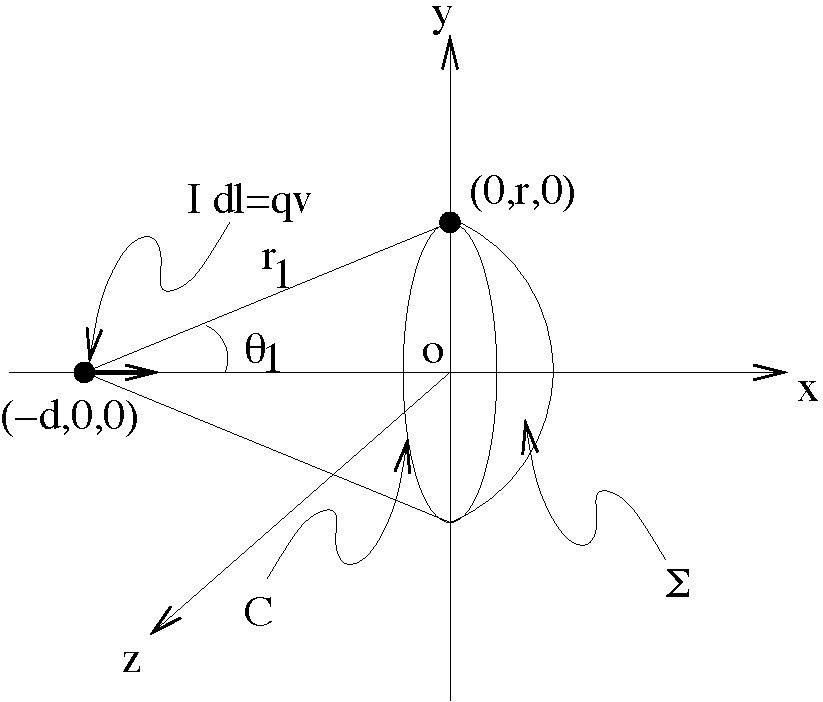
\includegraphics[width = 15cm]{m6}
    \caption{Calculation of magnetic field of a moving charge by
``generalized'' Ampere's law.}
  \end{figure}

Consider a surface $\Sigma$ whose boundary is the circle $C$ centered
at the origin and in Y-Z plane, and all points on $\Sigma$ have the
same distance $r_1$ to the moving charge at $(-d,0,0)$.  Apply Stoke's
Theorem,
\begin{eqnarray}
\int_{\Sigma} \vec{\nabla}\times\vec{B}\cdot d\vec{a} &=& \int_C
\vec{B}\cdot d\vec{l}\\
\textrm{while} \qquad\qquad \int_{\Sigma} \vec{\nabla}\times\vec{B}\cdot
d\vec{a} &=& \frac{1}{c}\int_{\Sigma} \frac{\partial \vec{E}}{\partial
t}\cdot d\vec{a}\nonumber\\
&=& \frac{1}{c}\frac{\partial}{\partial t}\int_{\Sigma} \vec{E}\cdot
d\vec{a}\\
\textrm{so}\qquad \int_C \vec{B}\cdot d\vec{l} &=&
\frac{1}{c}\frac{\partial}{\partial t}\int_{\Sigma} \vec{E}\cdot
d\vec{a}.
\end{eqnarray}

On the surface $\Sigma$, $E=q/r_1^2$ in radial direction (seen from
the moving charge).  So
\begin{eqnarray}
\int \vec{E}\cdot d\vec{a} &=& \frac{q}{r_1^2}\int da\nonumber\\
&=& \frac{q}{r_1^2}r_1^2\int_{0}^{\theta_1}\sin\theta d\theta
\int_0^{2\pi}d\phi\nonumber\\
&=& 2\pi q\left[\cos(0) - \cos(\theta_1)\right]\nonumber\\
&=& 2\pi q(1-\frac{d}{\sqrt{d^2+r^2}}).
\end{eqnarray}

Then, since $d(-d)/dt=v$,
\begin{eqnarray}
\frac{1}{c}\frac{\partial}{\partial t}\int_{\Sigma} \vec{E}\cdot
d\vec{a} &=& \frac{2\pi qv}{c}\frac{r^2}{(d^2+r^2)^{3/2}}\\
\int_C \vec{B}\cdot d\vec{l} &=& 2\pi rB\\
B&=& \frac{qvr}{c(r^2+d^2)^{3/2}}.
\end{eqnarray}


\section{Problem \thesection: General questions}
\subsection{Problem}
\begin{figure}[H]
    \centering
    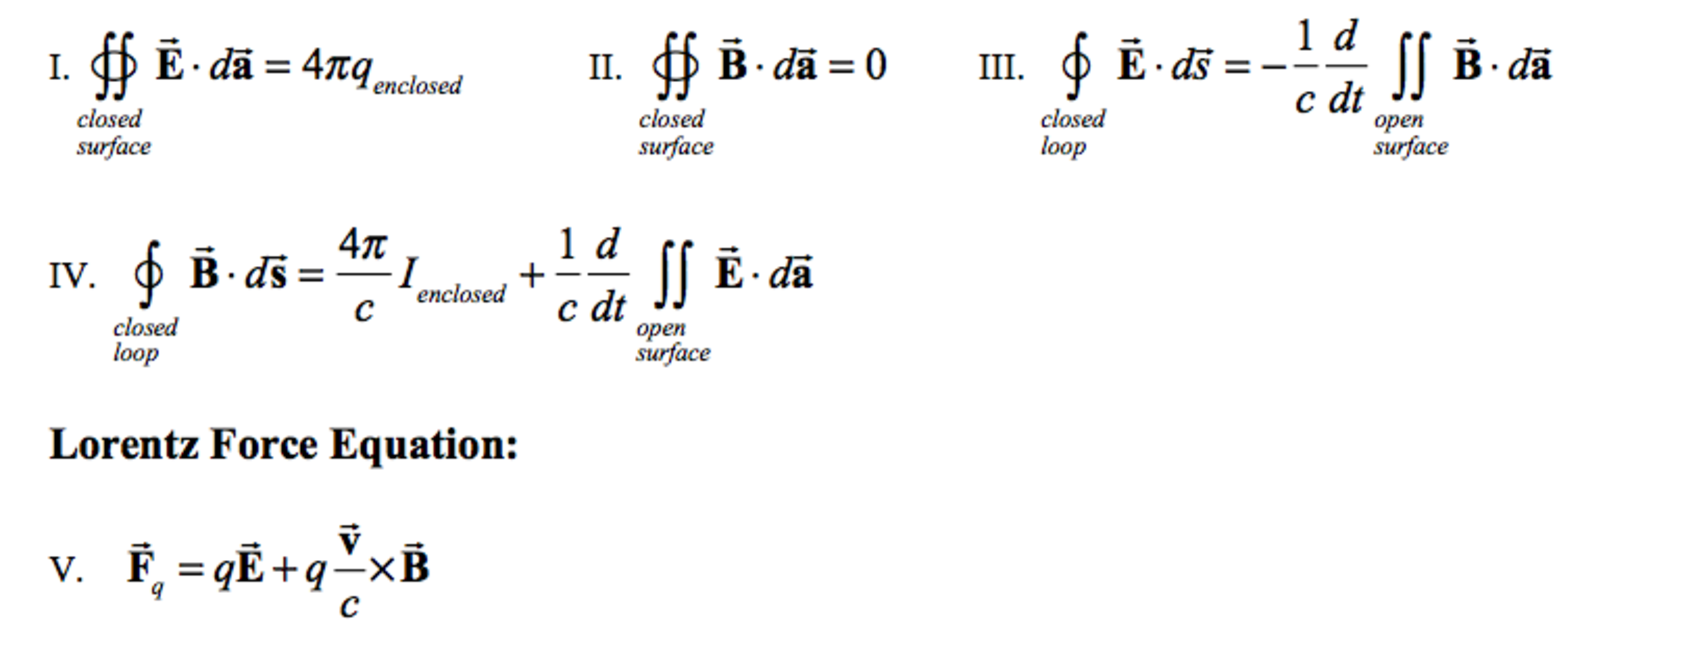
\includegraphics[width = 15cm]{eqns}
    \caption{Equations}
  \end{figure}
\begin{figure}[H]
    \centering
    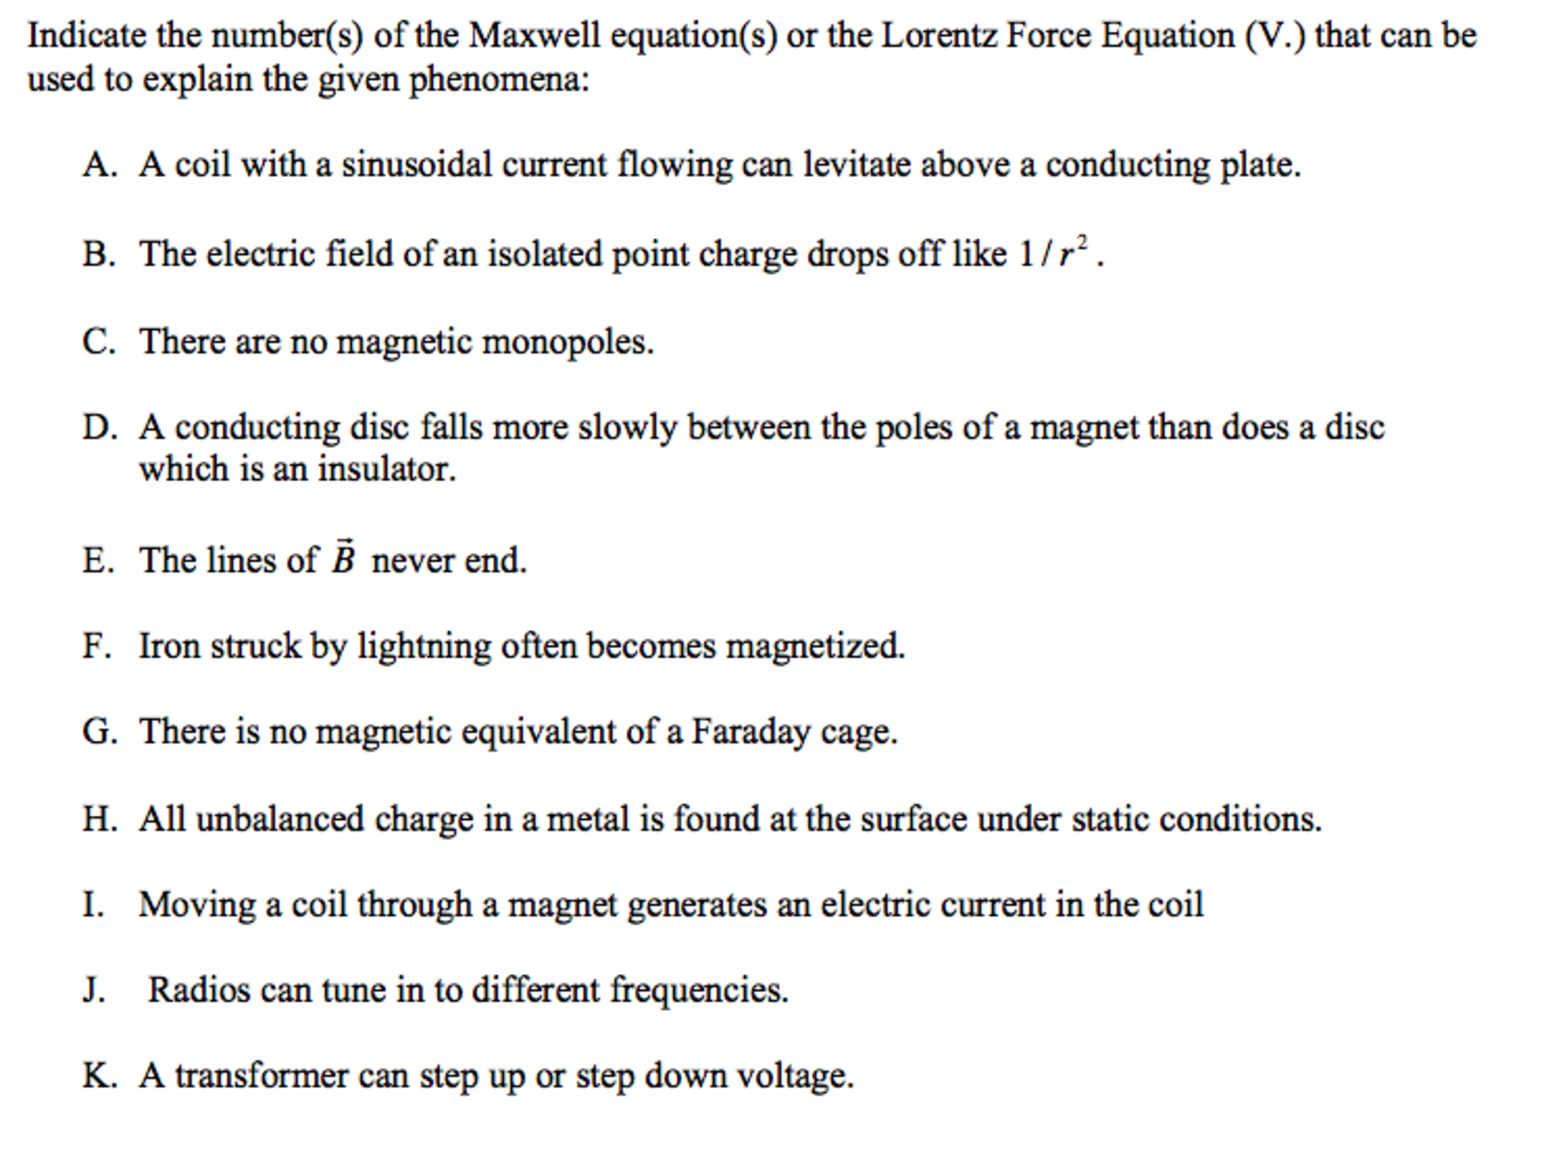
\includegraphics[width = 15cm]{max_gen}
    \caption{Maxwell's equations}
  \end{figure}
\subsection{Solution}
\begin{figure}[H]
    \centering
    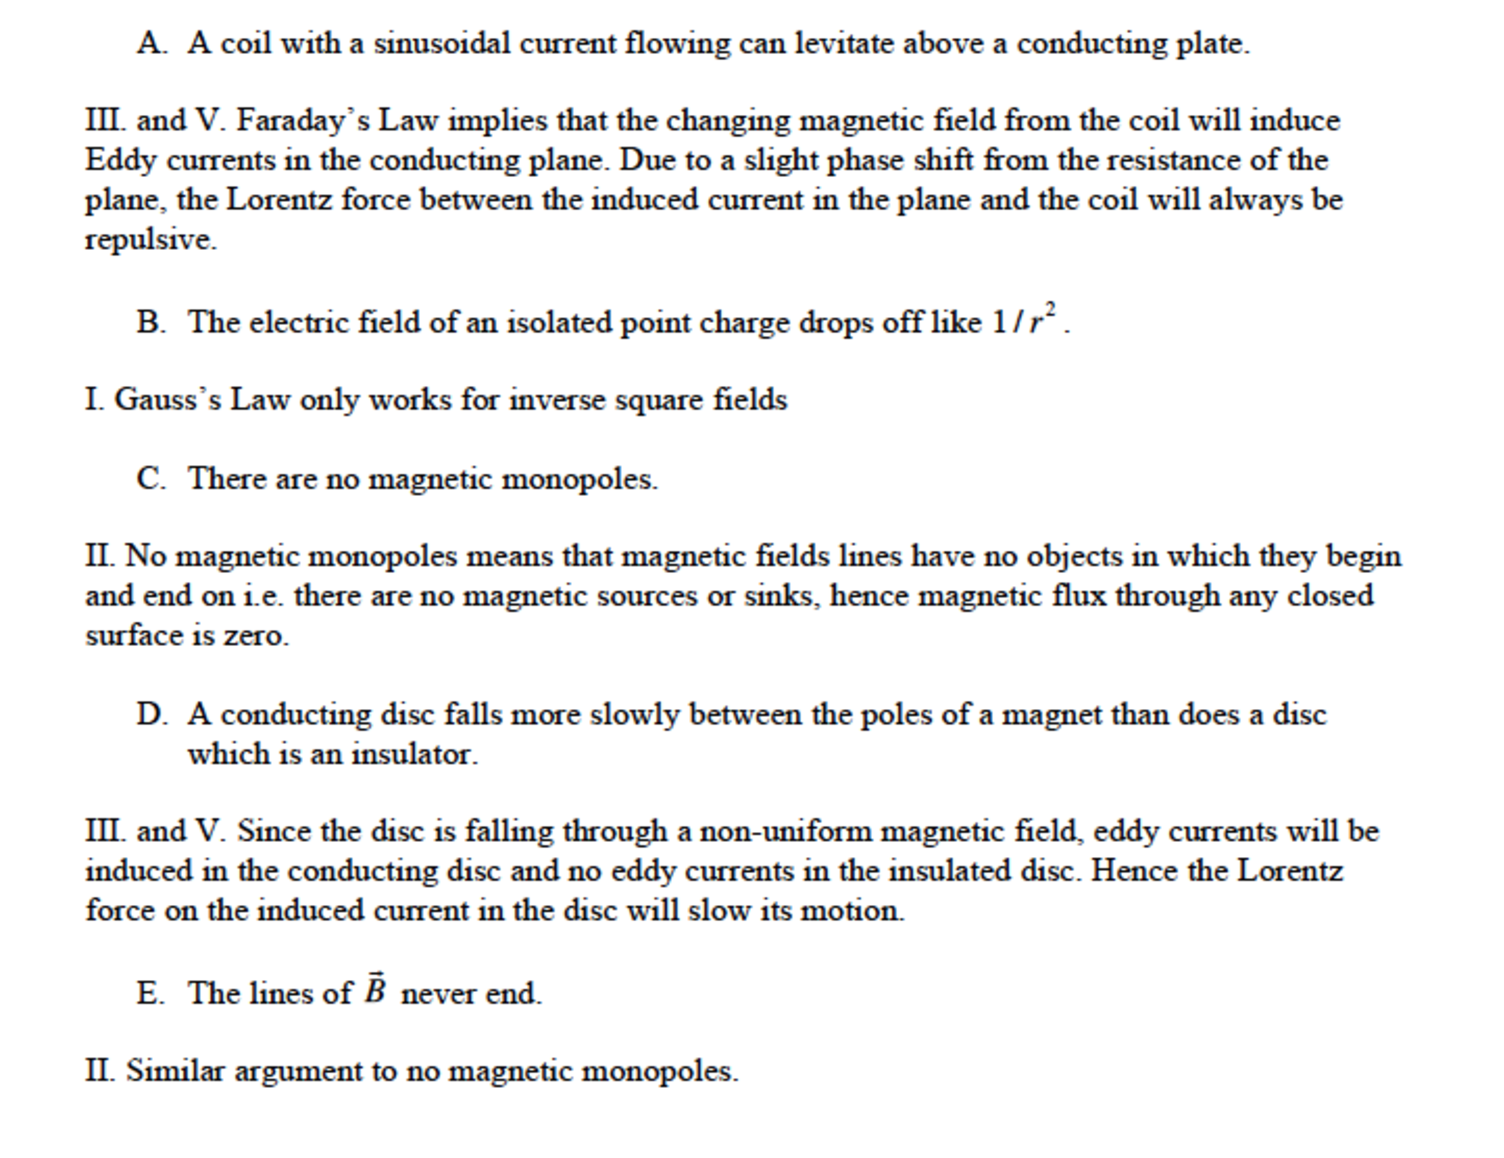
\includegraphics[width = 15cm]{max_gen_sola}
    \caption{Maxwell's equations}
  \end{figure}
  \begin{figure}[H]
    \centering
    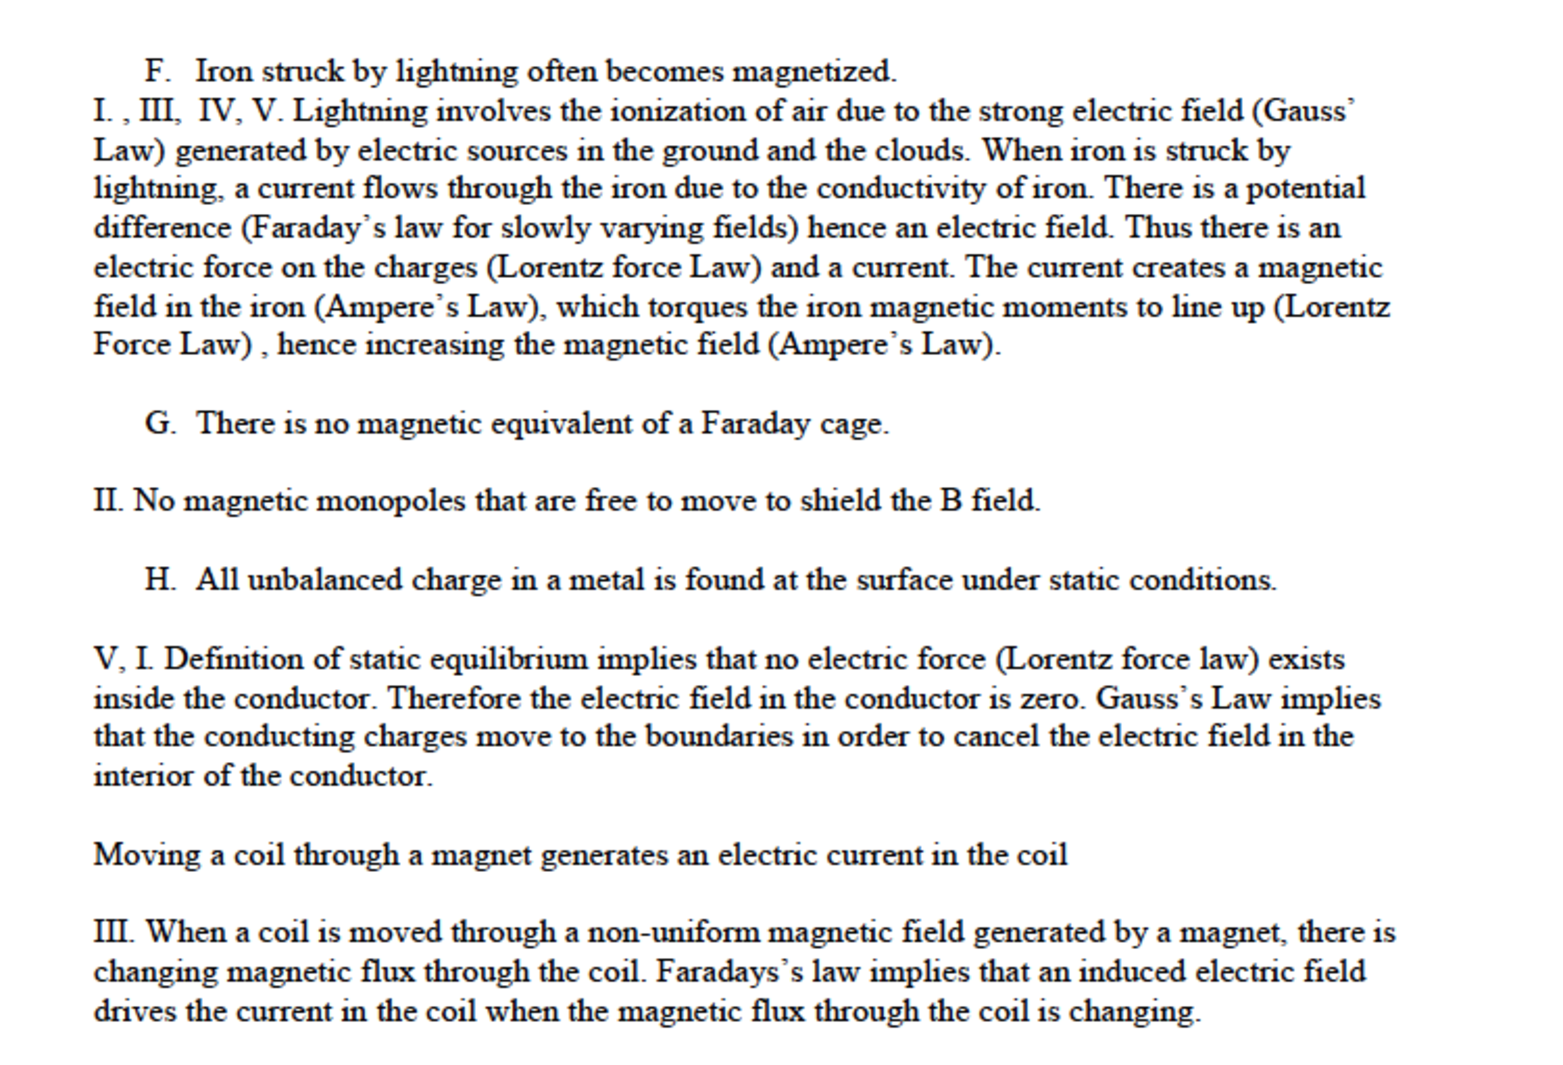
\includegraphics[width = 15cm]{max_gen_solb}
    \caption{Maxwell's equations}
  \end{figure}
  \begin{figure}[H]
    \centering
    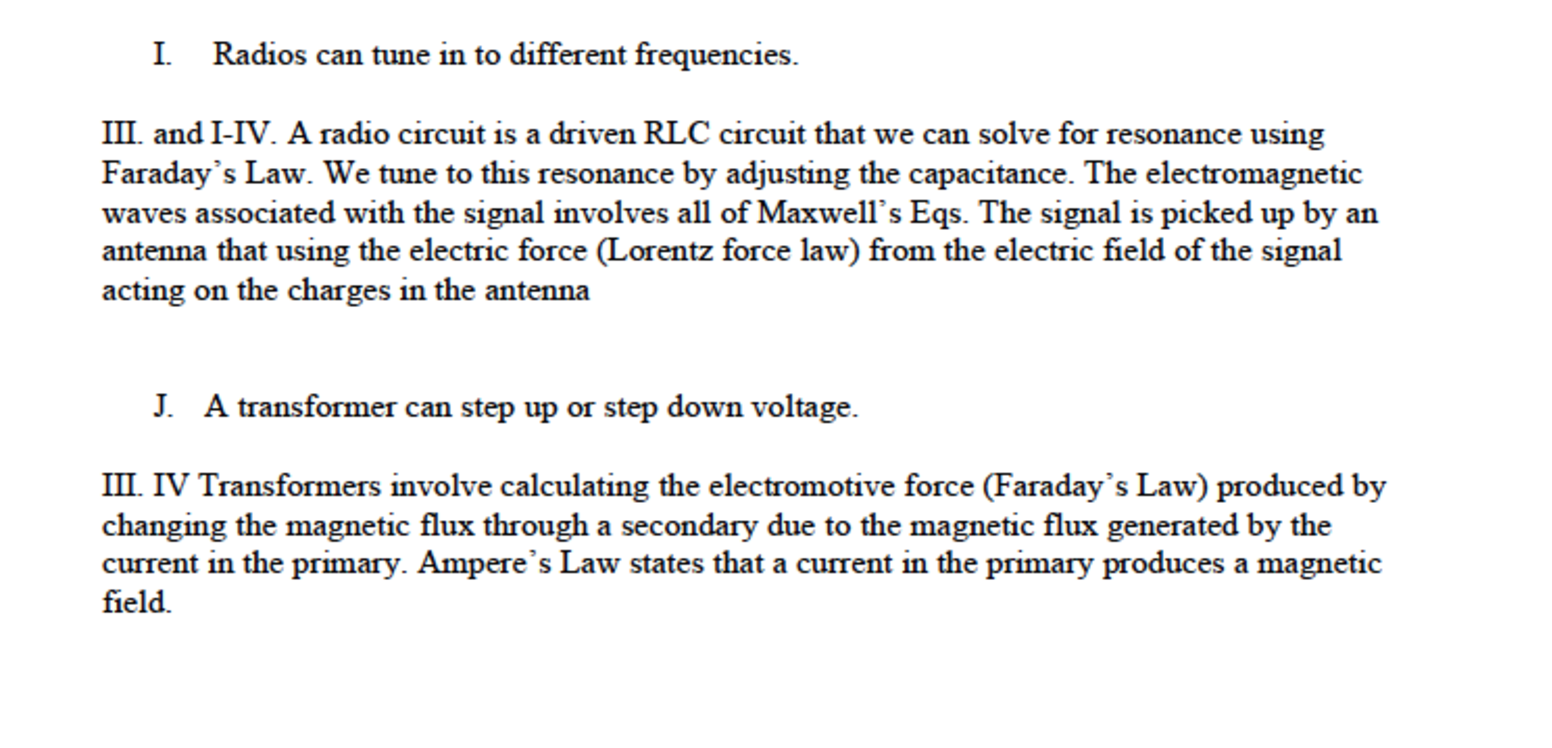
\includegraphics[width = 15cm]{max_gen_solc}
    \caption{Maxwell's equations}
  \end{figure}

\section{Problem \thesection: Purcell 9.1}
\subsection{Problem}

\begin{figure}[H]
    \centering
    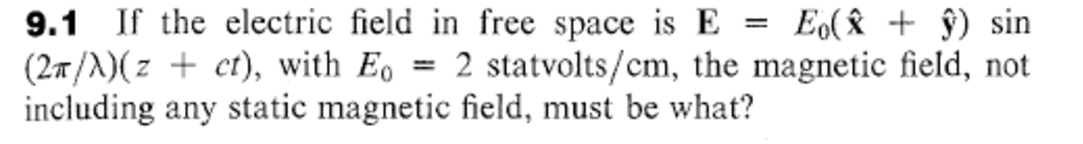
\includegraphics[width = 15cm]{pu901}
    \caption{Purcell 9.1}
  \end{figure}
  
\subsection{Solution}
  \begin{figure}[H]
    \centering
    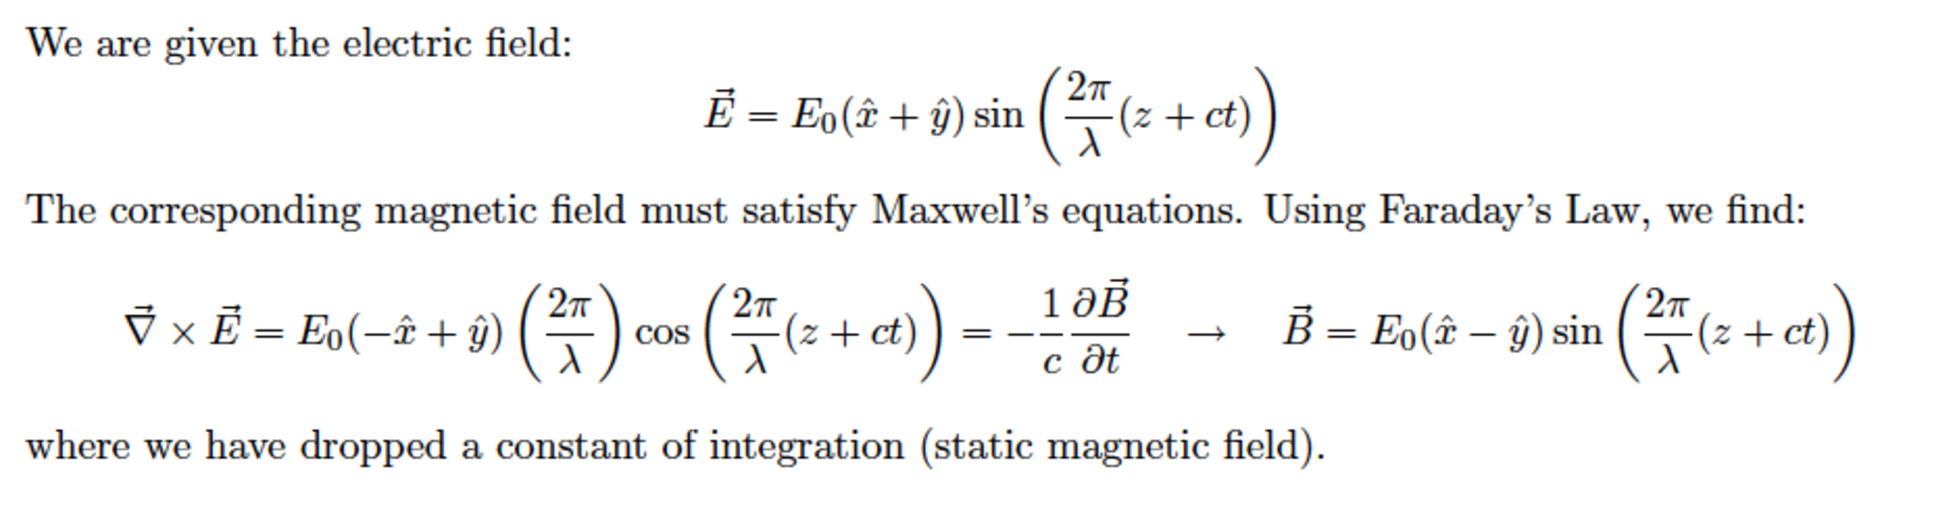
\includegraphics[width = 15cm]{solpu901}
    \caption{Solution Purcell 9.1}
  \end{figure}
\section{Problem \thesection: Purcell 9.5a}
\subsection{Problem}
 \begin{figure}[H]
    \centering
    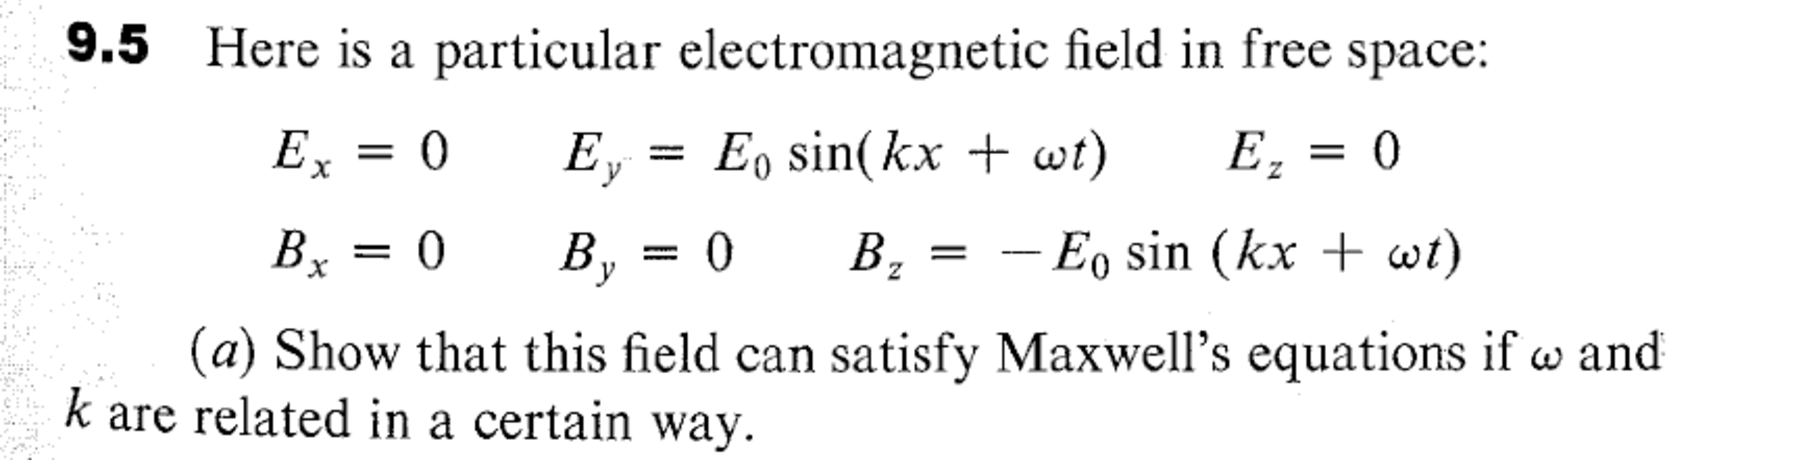
\includegraphics[width = 15cm]{pu905}
    \caption{Purcell 9.5}
  \end{figure}
\subsection{Solution}
 \begin{figure}[H]
    \centering
    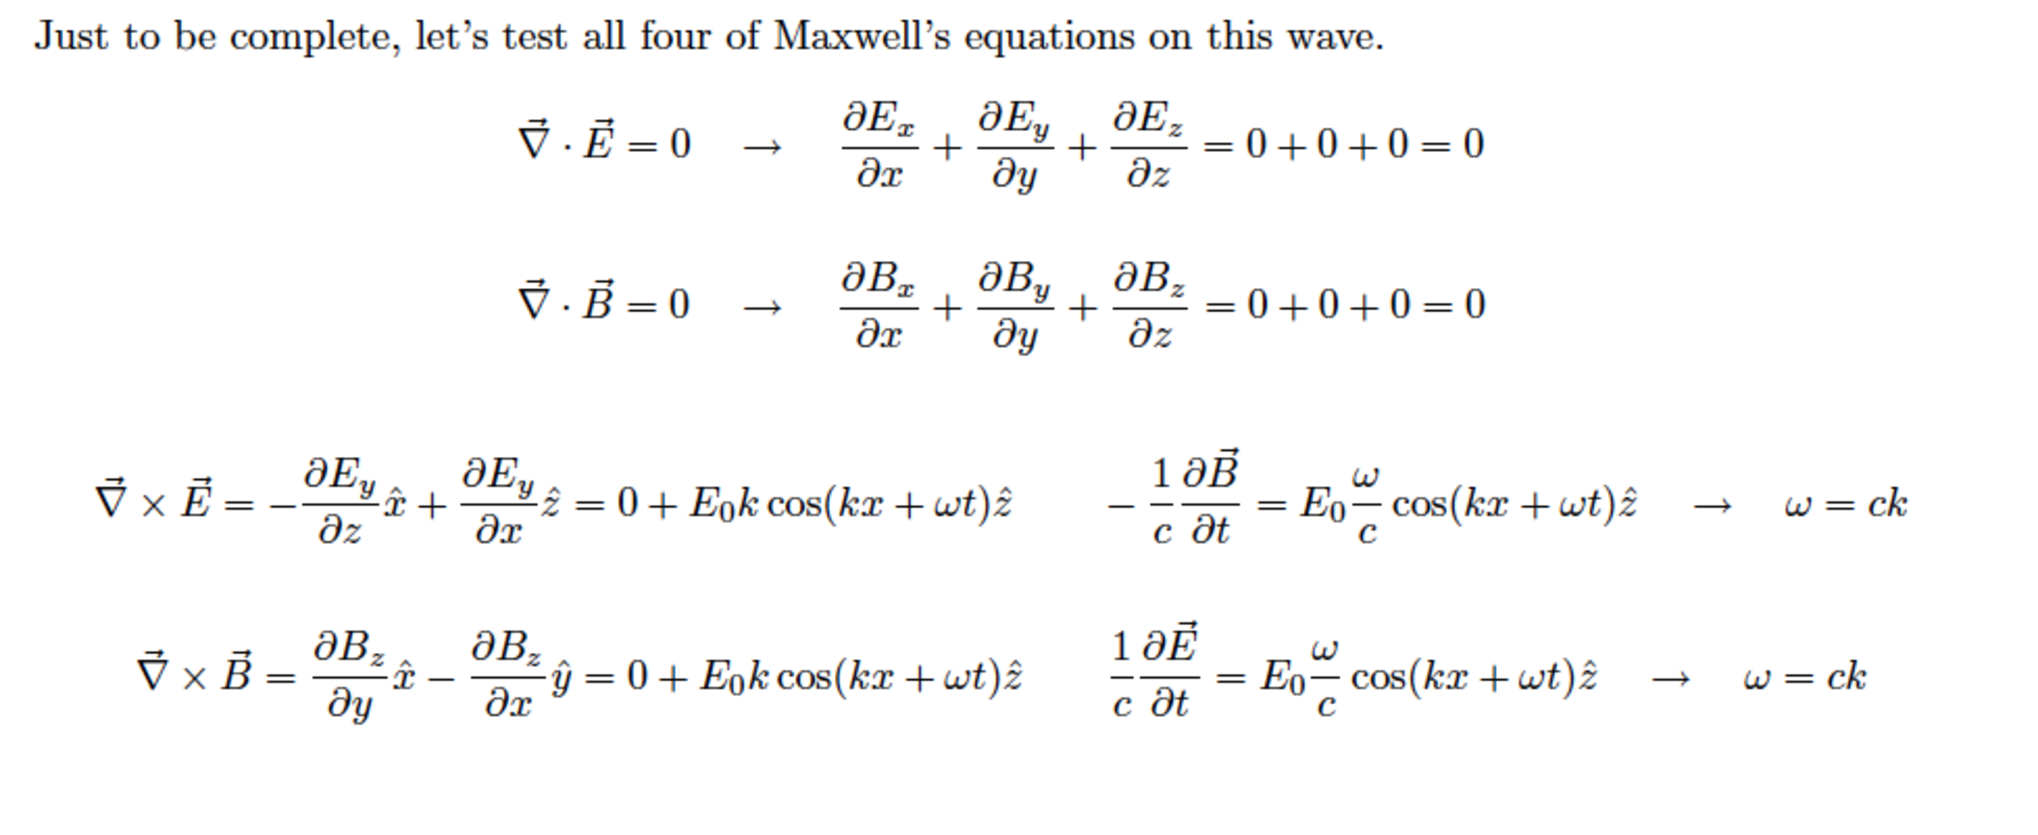
\includegraphics[width = 15cm]{solpu905a}
    \caption{Solution Purcell 9.5a}
  \end{figure}
\section{Problem \thesection: EM waves}
\subsection{Problem}
\begin{figure}[H]
    \centering
    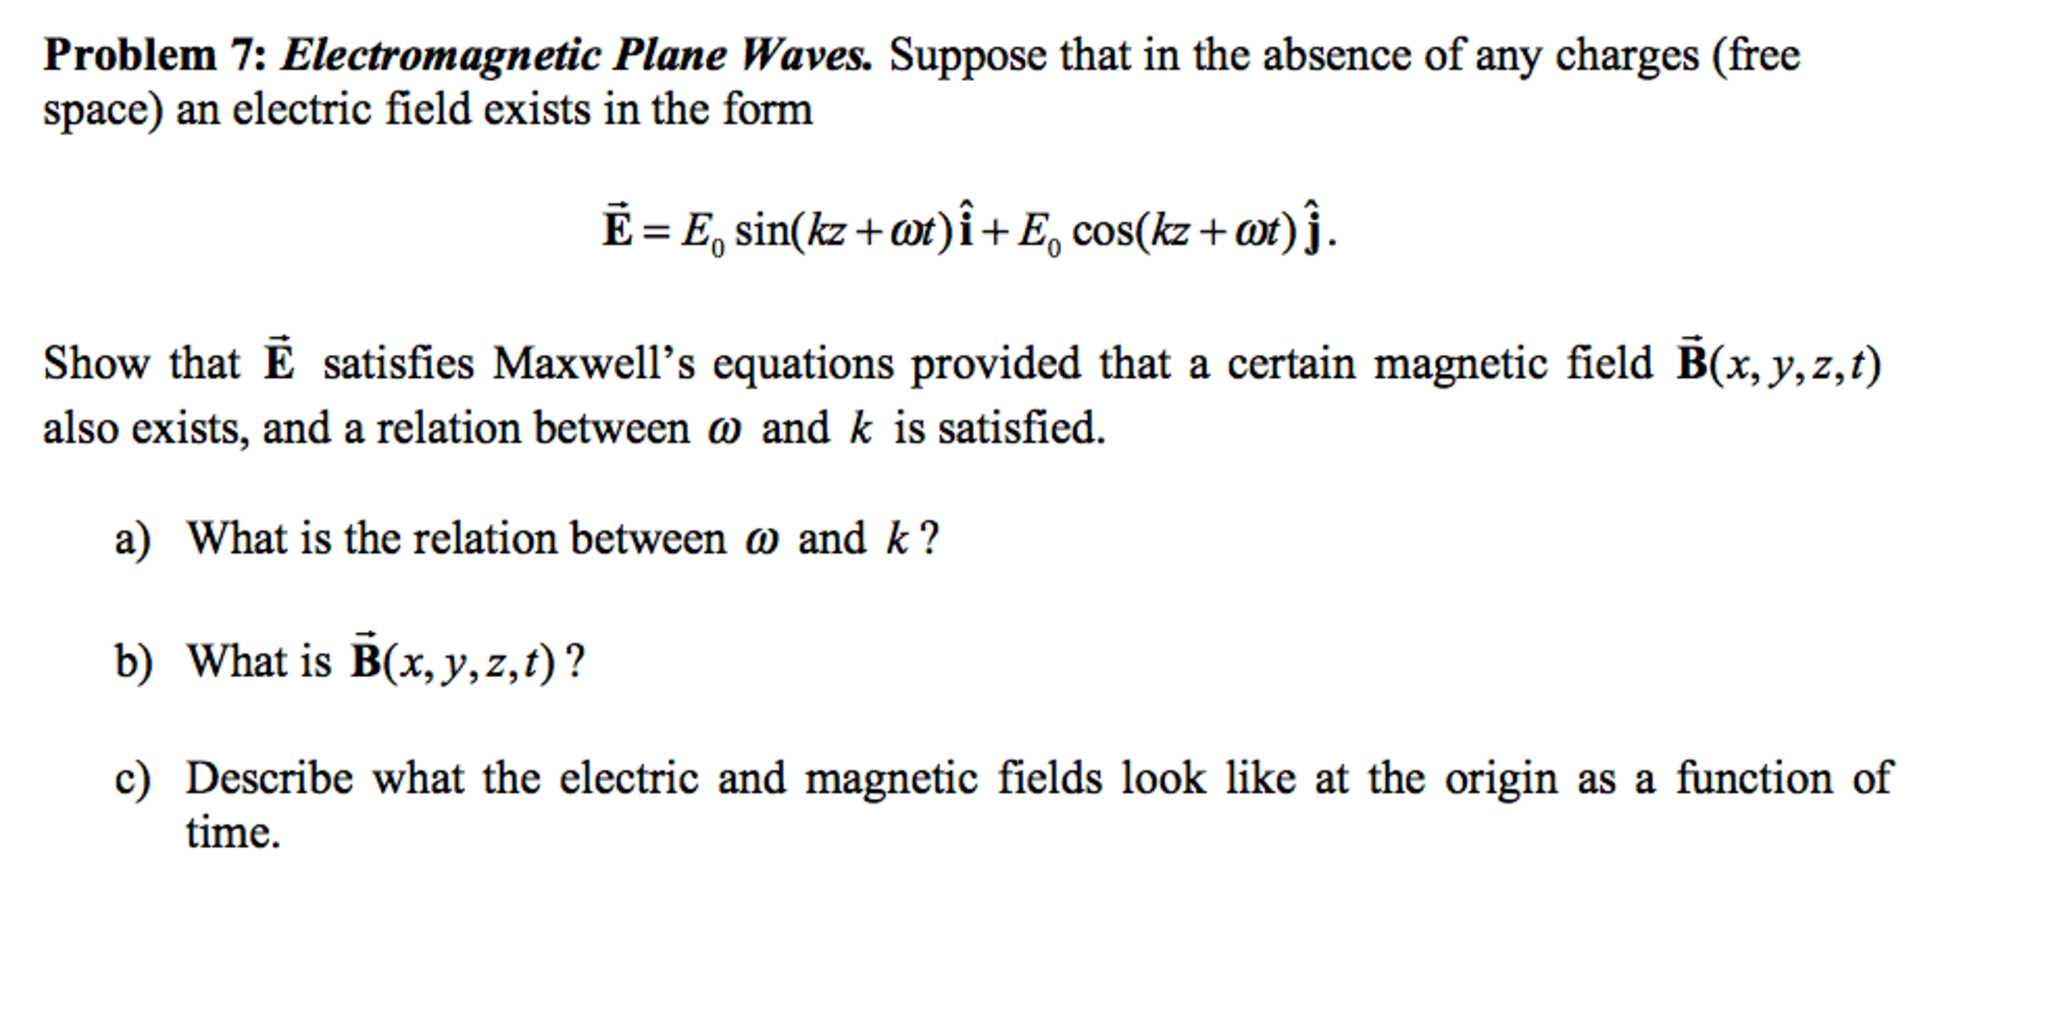
\includegraphics[width = 15cm]{waves2}
   \caption{Waves}
  \end{figure}
\subsection{Solution}
\begin{figure}[H]
    \centering
    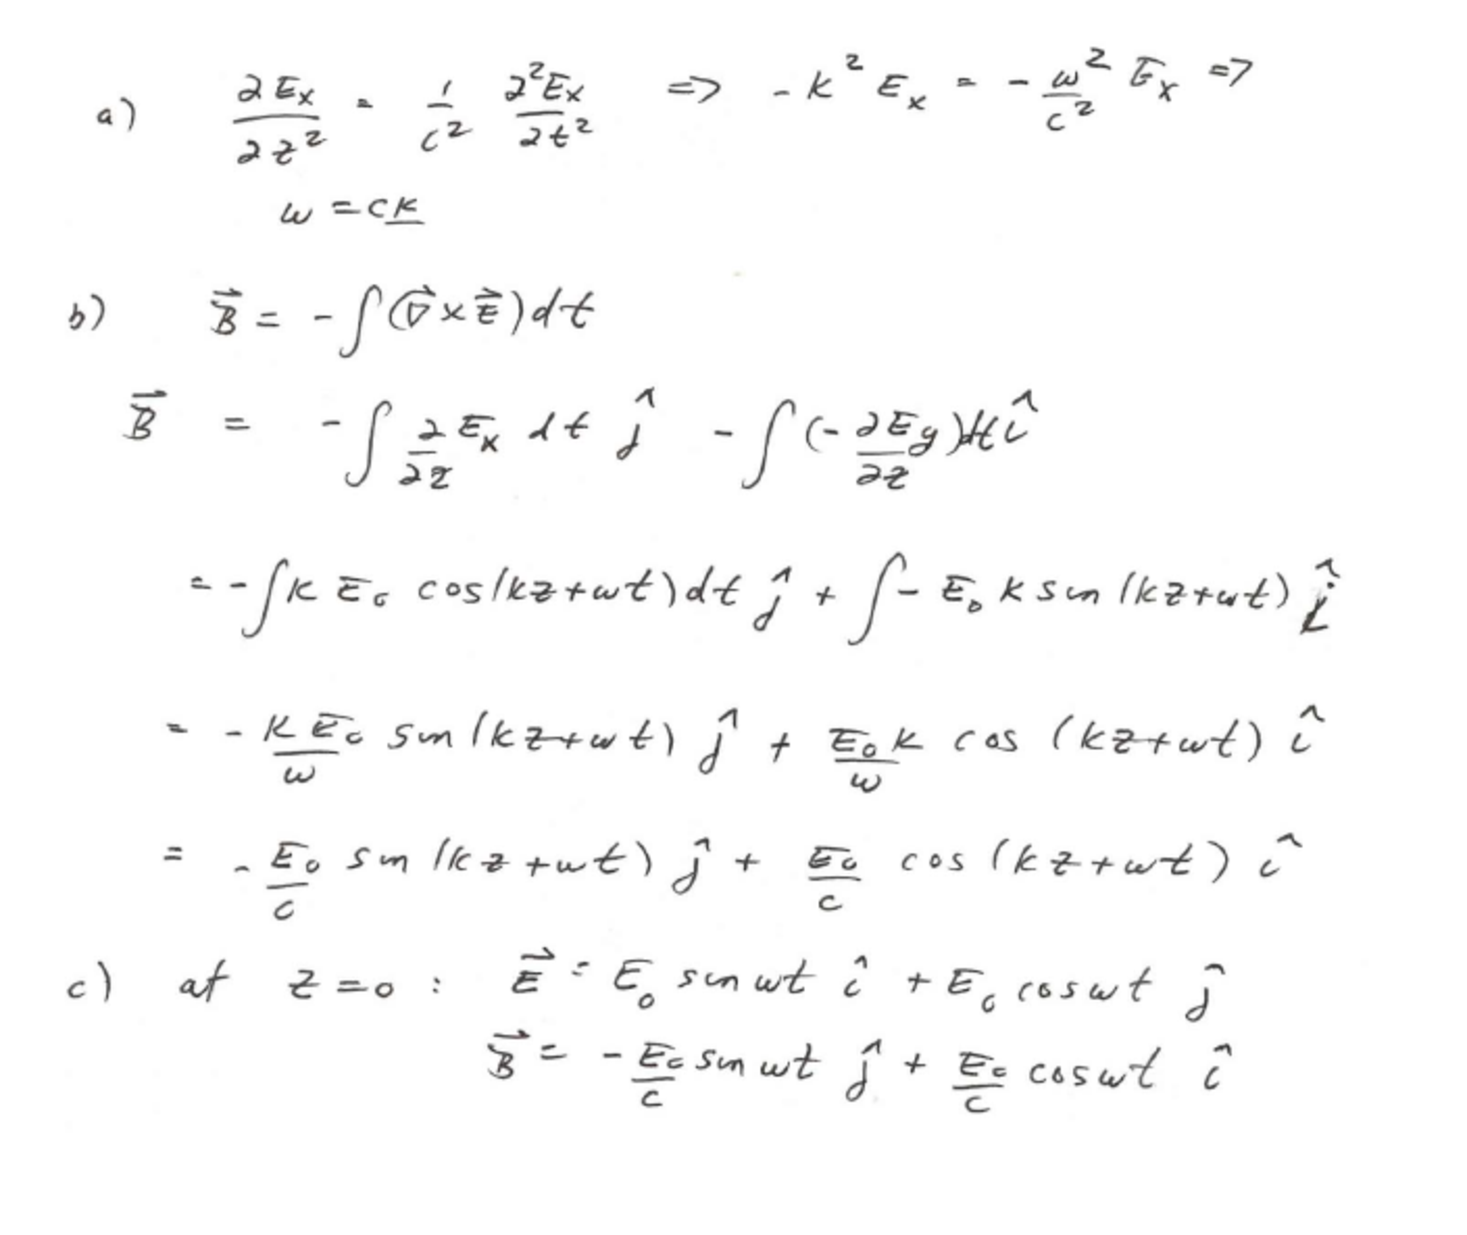
\includegraphics[width = 15cm]{waves2sola}
   \caption{Waves}
  \end{figure}
  \begin{figure}[H]
    \centering
    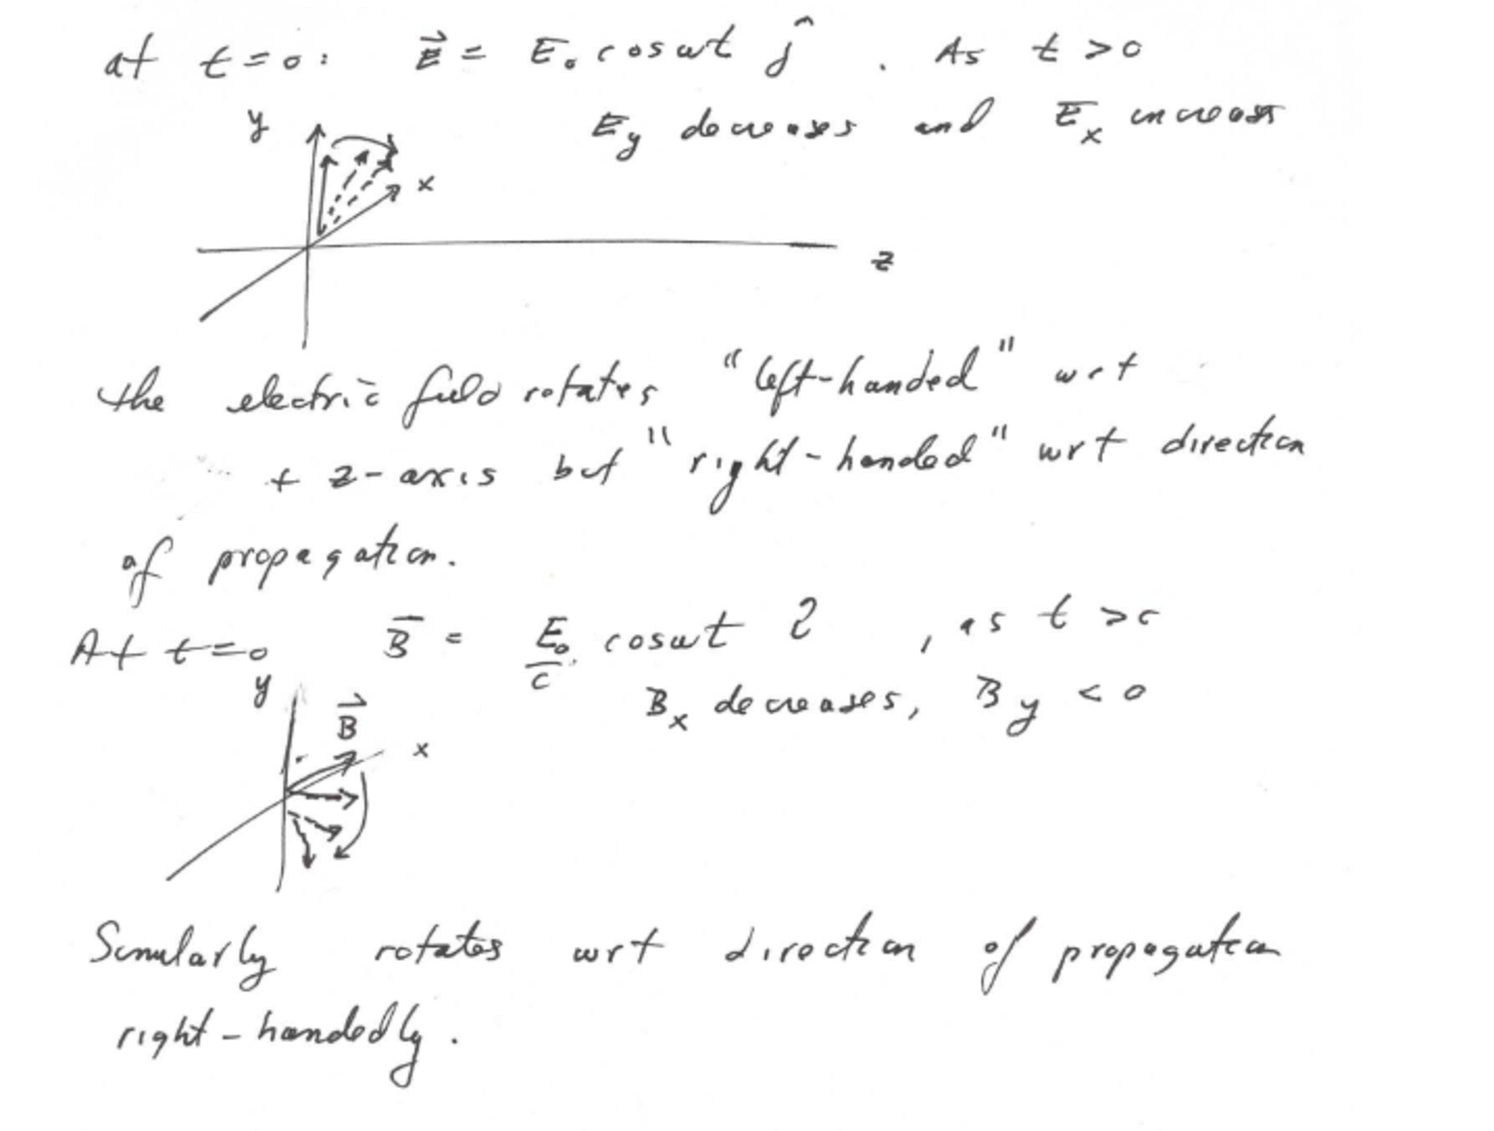
\includegraphics[width = 15cm]{waves2solb}
   \caption{Waves}
  \end{figure}
\section{Problem \thesection: Purcell 9.8}
\subsection{Problem}
\begin{figure}[H]
    \centering
    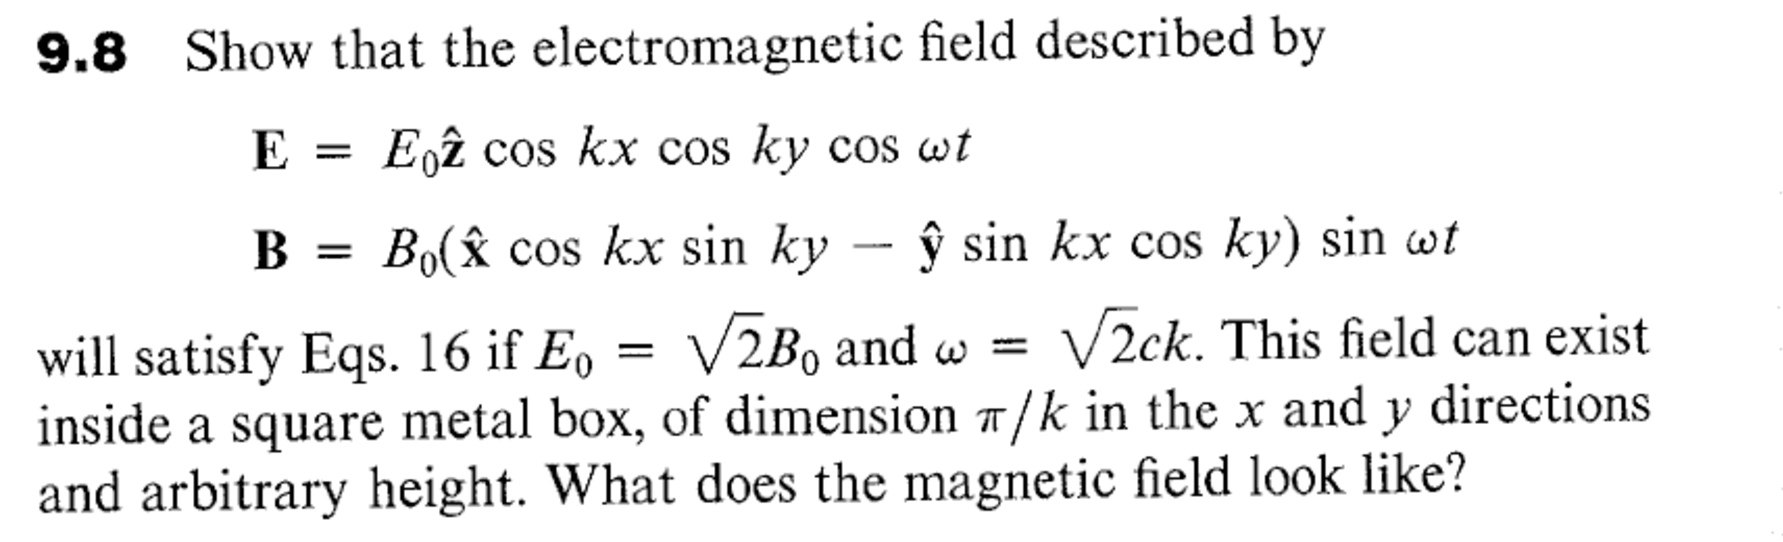
\includegraphics[width = 15cm]{pu908}
    \caption{Wave in a box}
  \end{figure}

\subsection{Solution}
For the EM field
\begin{eqnarray}
\vec{E} &=& \hat{z}E_0 \cos kx\cos ky\cos \omega t\\
\vec{B} &=&
B_0(\hat{x}\cos kx\sin ky-\hat{y}\sin kx\cos ky)\sin \omega t,
\end{eqnarray}
the two divergencelessness equations of Purcell eqs.(16)
\[ \vec{\nabla}\cdot\vec{E}=0 \,;\]
\[ \vec{\nabla}\cdot\vec{B}=0 \,,\]
can be easily verified.  The other two equations give
\begin{eqnarray}
\vec{\nabla}\times\vec{E}+\frac{1}{c}\frac{\partial \vec{B}}{\partial
t} &=& (\frac{\omega B_0}{c}-E_0 k)(\hat{x}\cos kx\sin ky
-\hat{y}\sin kx \cos ky)\cos \omega t =0\nonumber\\
\vec{\nabla}\times\vec{B}-\frac{1}{c}\frac{\partial \vec{E}}{\partial
t} &=& (\frac{E_0\omega}{c}-2B_0 k)\hat{z}\cos kx \cos ky \sin \omega
t =0\nonumber\\
or\;\;\;\;\;\;\; E_0 &=& \frac{\omega}{kc}B_0\\
E_0 &=& 2\frac{kc}{\omega}B_0.
\end{eqnarray}
So the condition is that
\begin{eqnarray}
\omega &=& \sqrt{2} ck\\
E_0 &=& \sqrt{2} B_0.
\end{eqnarray}

The magnetic field inside a square metal box of size $\pi/k$ is shown
in Figure \ref{fig:em2}.  Note that the box must run from $-\pi/(2k)$ to
$\pi/(2k)$ in both $x$ and $y$ in order to satisfy the boundary
condition that $E = 0$ on the box (which follows from the fact that
electric fields vanish on conductors).

\begin{figure}[H]
    \centering
    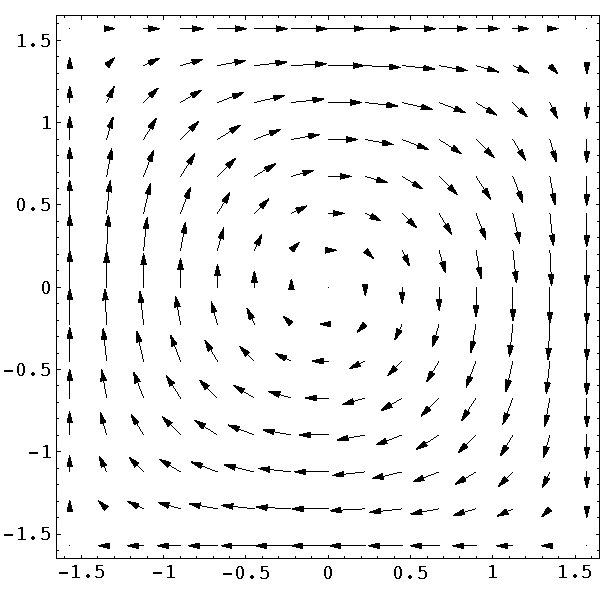
\includegraphics[width = 9cm]{em2}
    \caption{The magnetic field inside a squre metal box at
$t=\pi/2\omega$.  The horizontal axis is $kx$ and vertical axis $ky$.}
  \end{figure}

\section{Problem \thesection: Galilean Transformation of Maxwell's Wave Equation}
\subsection{Problem}

Observers in frame $F$ take 8.022 and derive Maxwell's wave equation:
$$\nabla^2\vec{E} - \frac{1}{c^2} \frac{\partial^2\vec{E}}{\partial t^2} = 0$$
For simplicity and specificity, assume that $\vec{E} = E(x,t)\, \hat{y}$, and therefore, the wave equation reduces to:
$$\frac{\partial^2E}{\partial x^2} - \frac{1}{c^2} \frac{\partial^2E}{\partial t^2} = 0$$
The goal of this problem is to understand what form the wave equation would have for observers in another inertial frame $F'$ frame moving along the $x$ axis with speed $v$.  The Galilean transformation of coordinates between the two frames is:
$$x' = x - vt$$
$$t' = t~~~~~~~$$


\noindent
a. Use the chain rule to show that
$$\frac{\partial E}{\partial x} = \frac{\partial E}{\partial x'}$$


\noindent
b. Use the chain rule to show that
$$\frac{\partial E}{\partial t} = -v \frac{\partial E}{\partial x'} + \frac{\partial E}{\partial t'}$$


\noindent
c. Use the results of parts (a) and (b) to show that the original wave equation in $F$ transforms to
$$\frac{\partial^2E}{\partial x'^2} - \frac{1}{c^2} \frac{\partial^2E}{\partial t'^2} = -\frac{2v}{c^2} \frac{\partial^2E}{\partial x' \partial t'} + \frac{v^2}{c^2} \frac{\partial^2E}{\partial x'^2}$$
in frame $F'$.


\noindent
d. Show that in frame $F'$ a person computing the speed of waves, $V$, governed by the modified Maxwell wave equation, would find $V = v \pm c$.  You may simply assume that the waves are of the form
$$E(x' \pm Vt')$$
where $E$ is an arbitrary function.

\subsection{Solution}

a. Using chain rule we get,
$$\frac{\partial E}{\partial x} = \frac{\partial x'}{\partial x}\frac{\partial E}{\partial x'} + \frac{\partial t'}{\partial x}\frac{\partial E}{\partial t'}$$
Note that
$$\frac{\partial x'}{\partial x} = 1 \quad \mbox{and} \quad  \frac{\partial t'}{\partial x} = 0$$
Hence,
$$\frac{\partial E}{\partial x} = \frac{\partial E}{\partial x'}$$


b. In this case
$$\frac{\partial E}{\partial t} = \frac{\partial x'}{\partial t}\frac{\partial E}{\partial x'} + \frac{\partial t'}{\partial t}\frac{\partial E}{\partial t'}$$
We also know that
$$\frac{\partial x'}{\partial t} = -v \quad \mbox{and} \quad  \frac{\partial t'}{\partial t} = 1$$
Therefore,
$$\frac{\partial E}{\partial t} = -v \frac{\partial E}{\partial x'} + \frac{\partial E}{\partial t'}$$

c. Using the result of part (a) we get,
$$\frac{\partial^2E}{\partial x^2}=\frac{\partial }{\partial x} ( \frac{\partial E}{\partial x'})= \frac{\partial }{\partial x'}(\frac{\partial E}{\partial x'}) $$
Similarly replacing in the result of part (b) $E$ by ${\partial E}/\partial t$ we get
$$\frac{\partial^{2} E}{\partial t^{2}} = (-v \frac{\partial }{\partial x'} + \frac{\partial }{\partial t'}) ( \frac{\partial E}{\partial t} )$$
Using the result of part (b) again we get (after some algebra)
$$ \frac{1}{c^2} \frac{\partial^2E}{\partial t^2}= \frac{1}{c^2} \frac{\partial^2E}{\partial t'^2}  -\frac{2v}{c^2} \frac{\partial^2E}{\partial x' \partial t'} + \frac{v^2}{c^2} \frac{\partial^2E}{\partial x'^2}$$
Hence, the wave equation in fame $F'$ is given by,
$$\frac{\partial^2E}{\partial x'^2} - \frac{1}{c^2} \frac{\partial^2E}{\partial t'^2} = -\frac{2v}{c^2} \frac{\partial^2E}{\partial x' \partial t'} + \frac{v^2}{c^2} \frac{\partial^2E}{\partial x'^2}$$


d. Substituting the given ansatz into the wave equation of $F'$ we get,
$$(1 - {V^{2}\over c^{2}}) E''(x' \pm Vt') = \mp{2 vV \over c^{2}} E''(x' \pm Vt') - {v^{2}\over c^{2}}E''(x' \pm Vt')$$
Hence, the assumed anastz is a solution if
$$1 = {1\over c^{2}}( V \mp v)^{2} $$
This implies the speed of the wave in frame $F'$ is $c\pm v$. It is known from experiments that the speed of light in vacuum is frame independent. But just now we had shown that EM waves in frame $F'$ (according to Galilean relativity) is $c\pm v$. Hence, it is clear that ``Galilean/Newtonian relativity'' is not consistent with Maxwell's equation. This is why we need Einstein's theory of special relativity.

\section{Problem \thesection: Optional: loop antenna}
\subsection{Problem}
\begin{figure}[H]
    \centering
    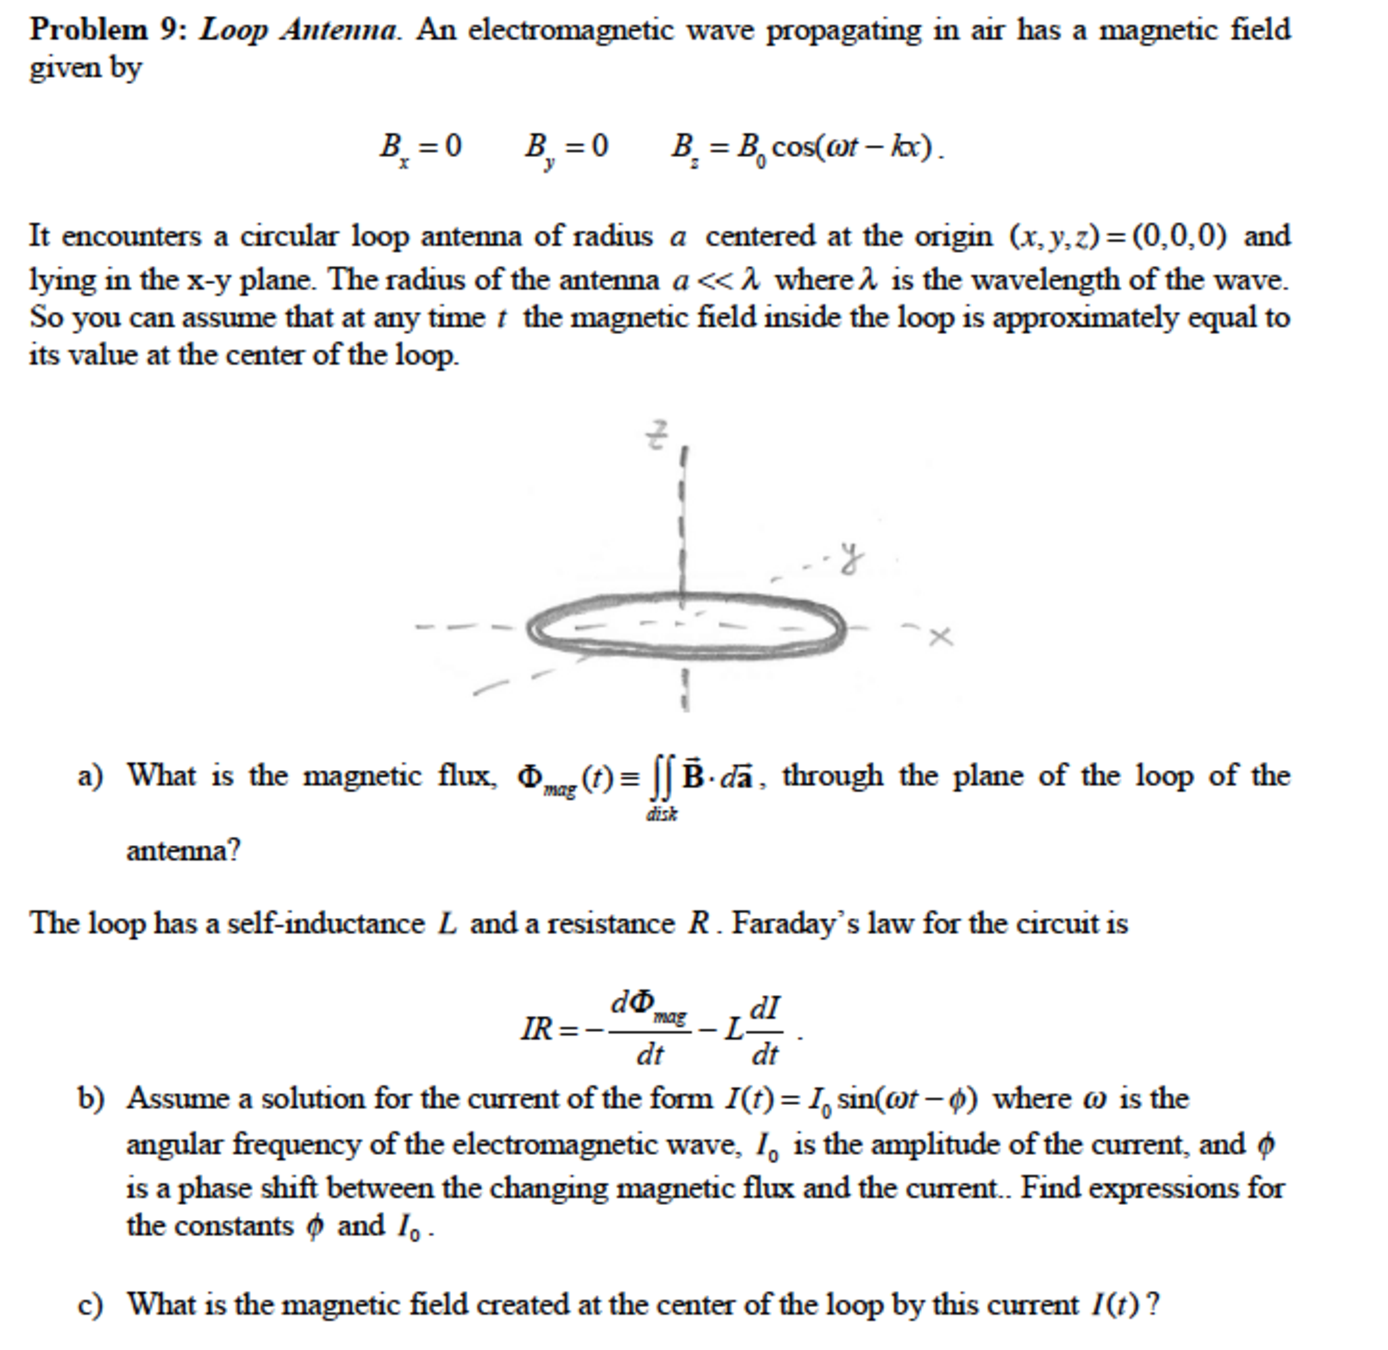
\includegraphics[width = 15cm]{loopantenna}
    \caption{Antenna}
  \end{figure}
\section{Problem \thesection: Optional --- Magnetic monopole: experiments}
\subsection{Problem}

 \begin{figure}[H]
    \centering
    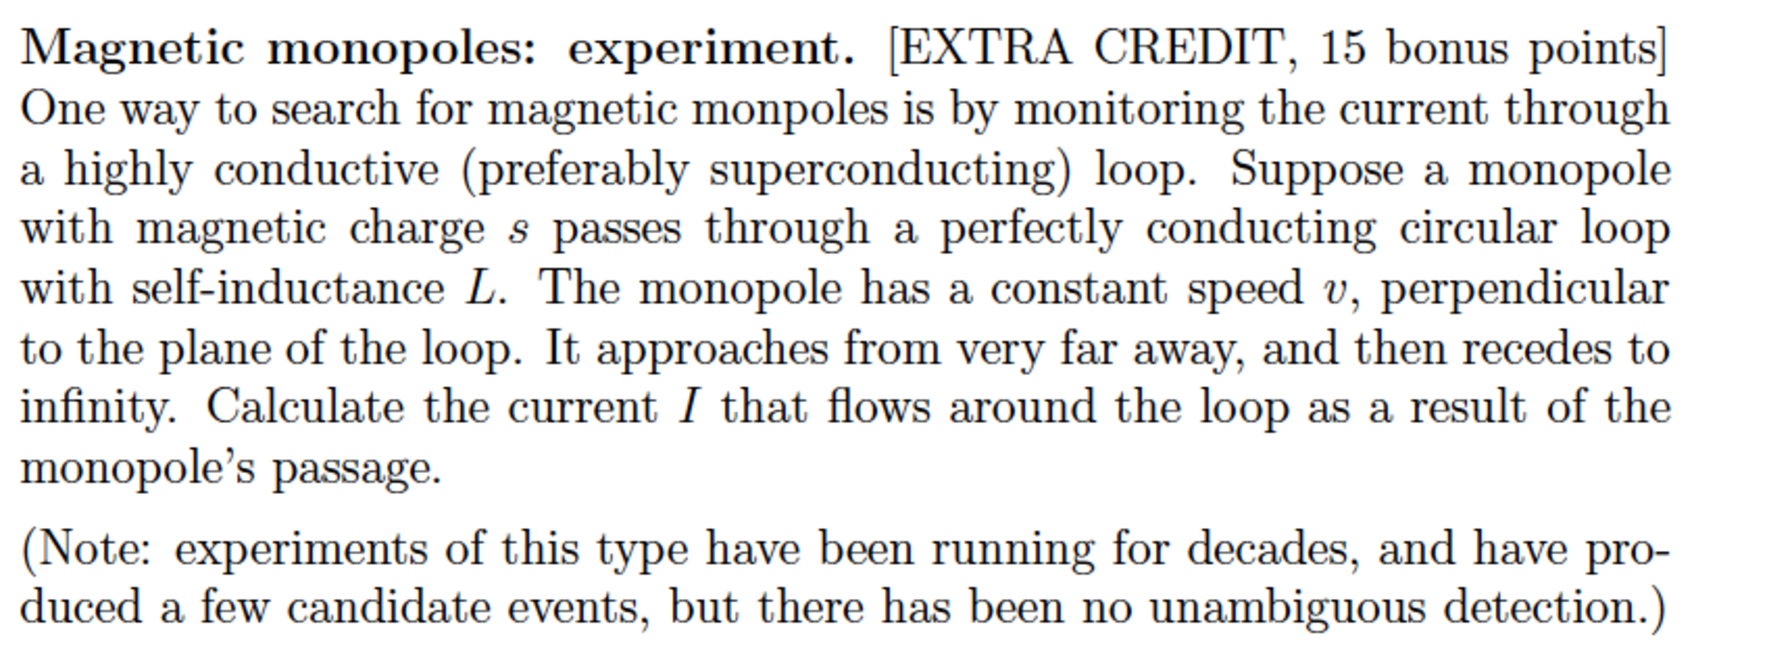
\includegraphics[width = 15cm]{monopoles}
    \caption{Magnetic monopole}
  \end{figure}

\subsection{Solution}

 \begin{figure}[H]
    \centering
    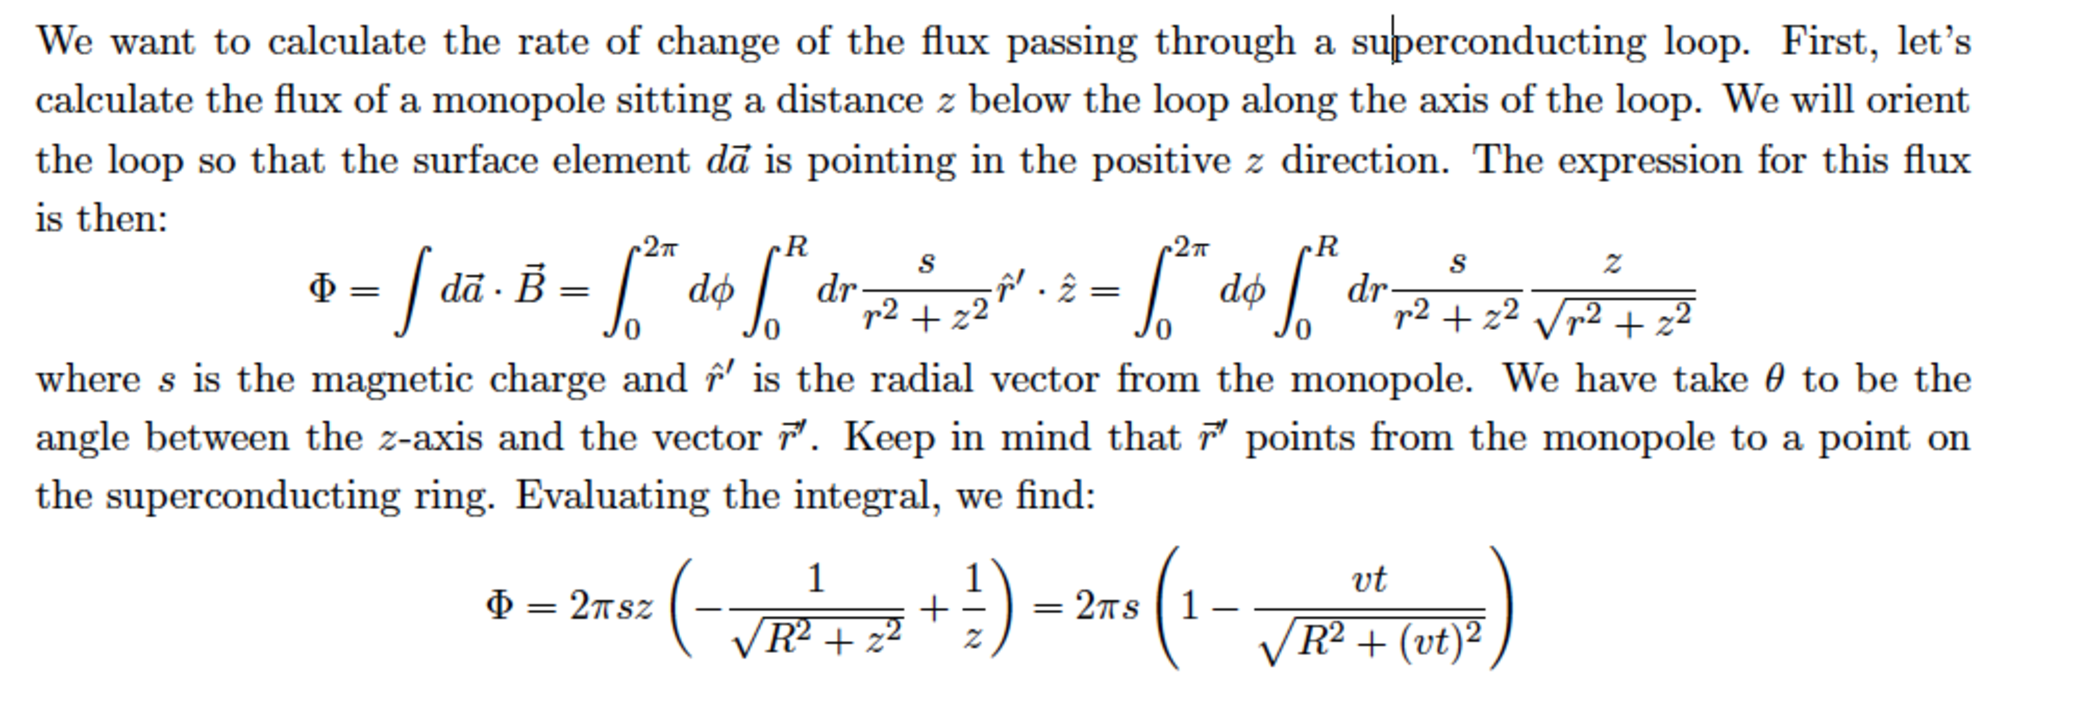
\includegraphics[width = 15cm]{mono_sol_a}
    \caption{Magnetic monopole}
\end{figure}

 \begin{figure}[H]
    \centering
    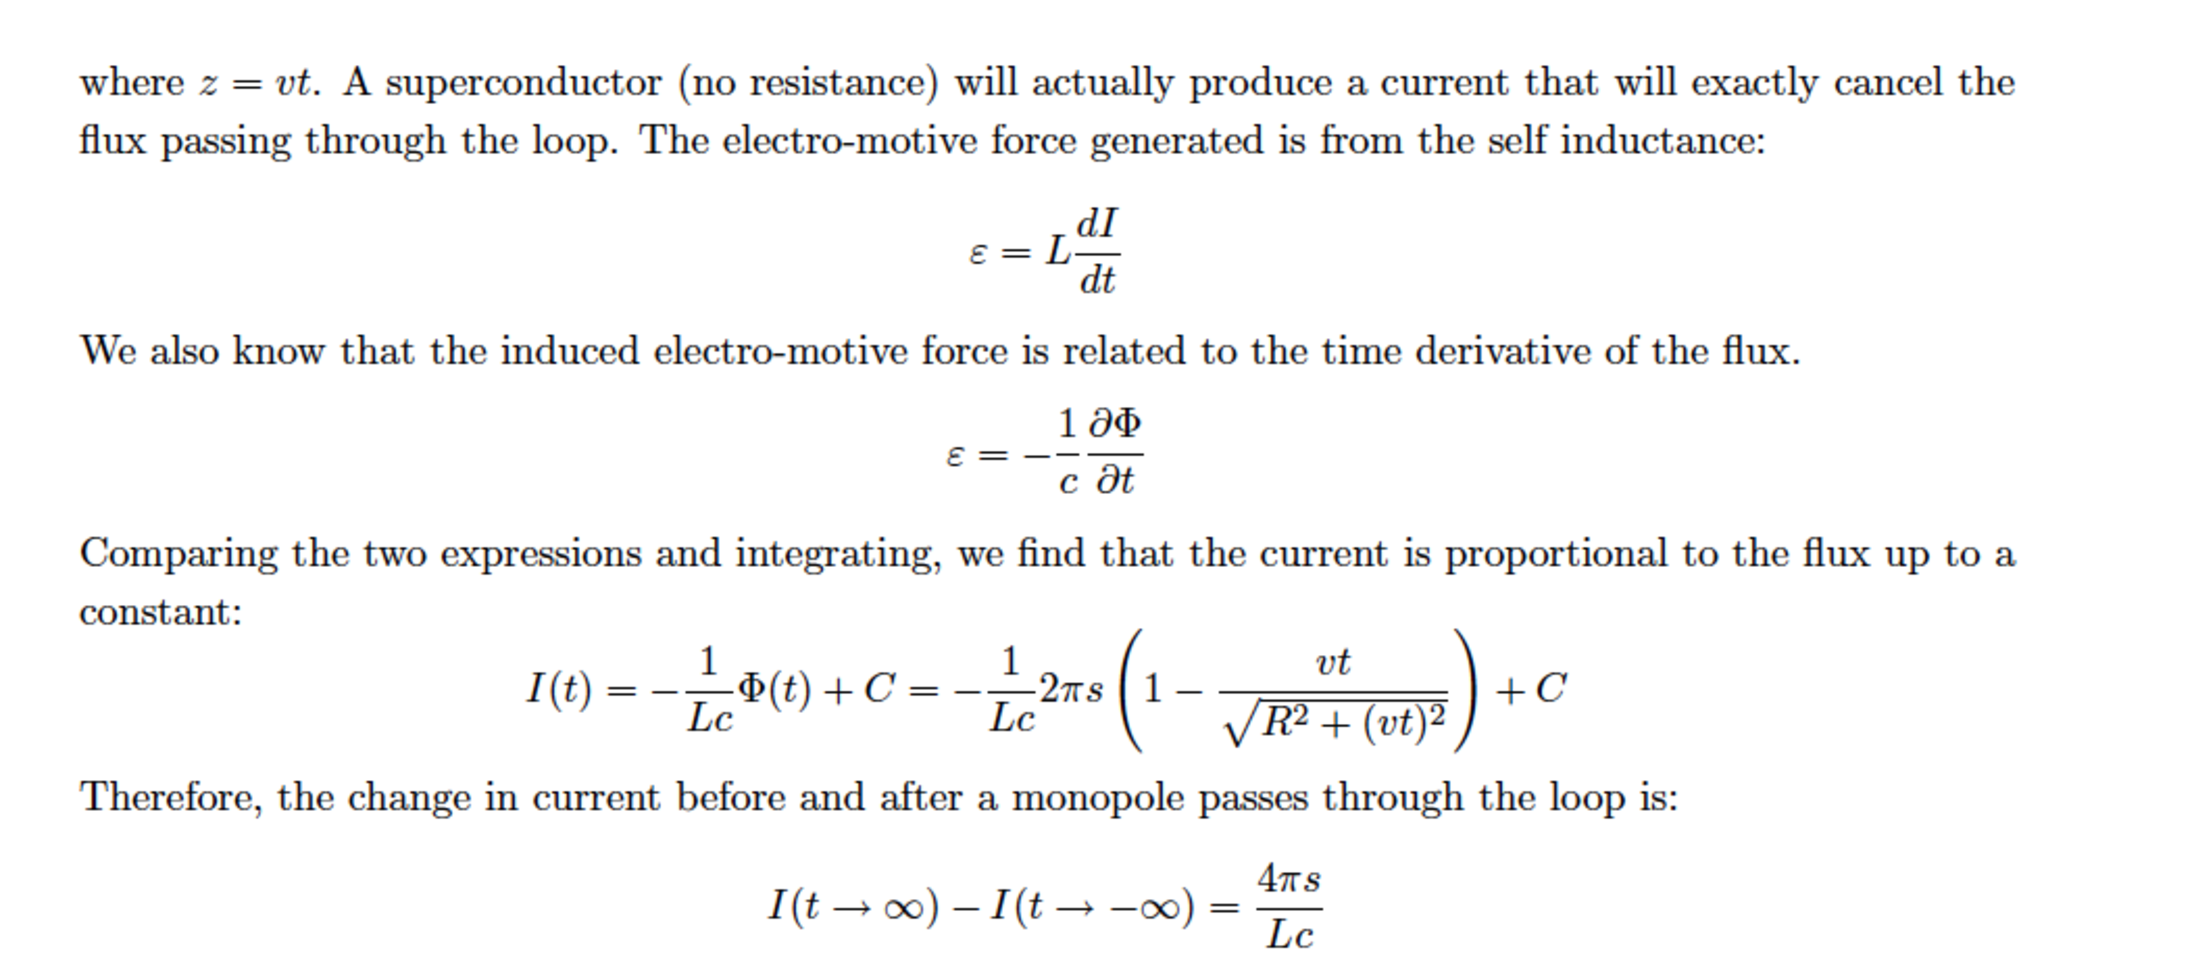
\includegraphics[width = 15cm]{mono_sol_b}
    \caption{Magnetic monopole}
\end{figure}

 \begin{figure}[H]
    \centering
    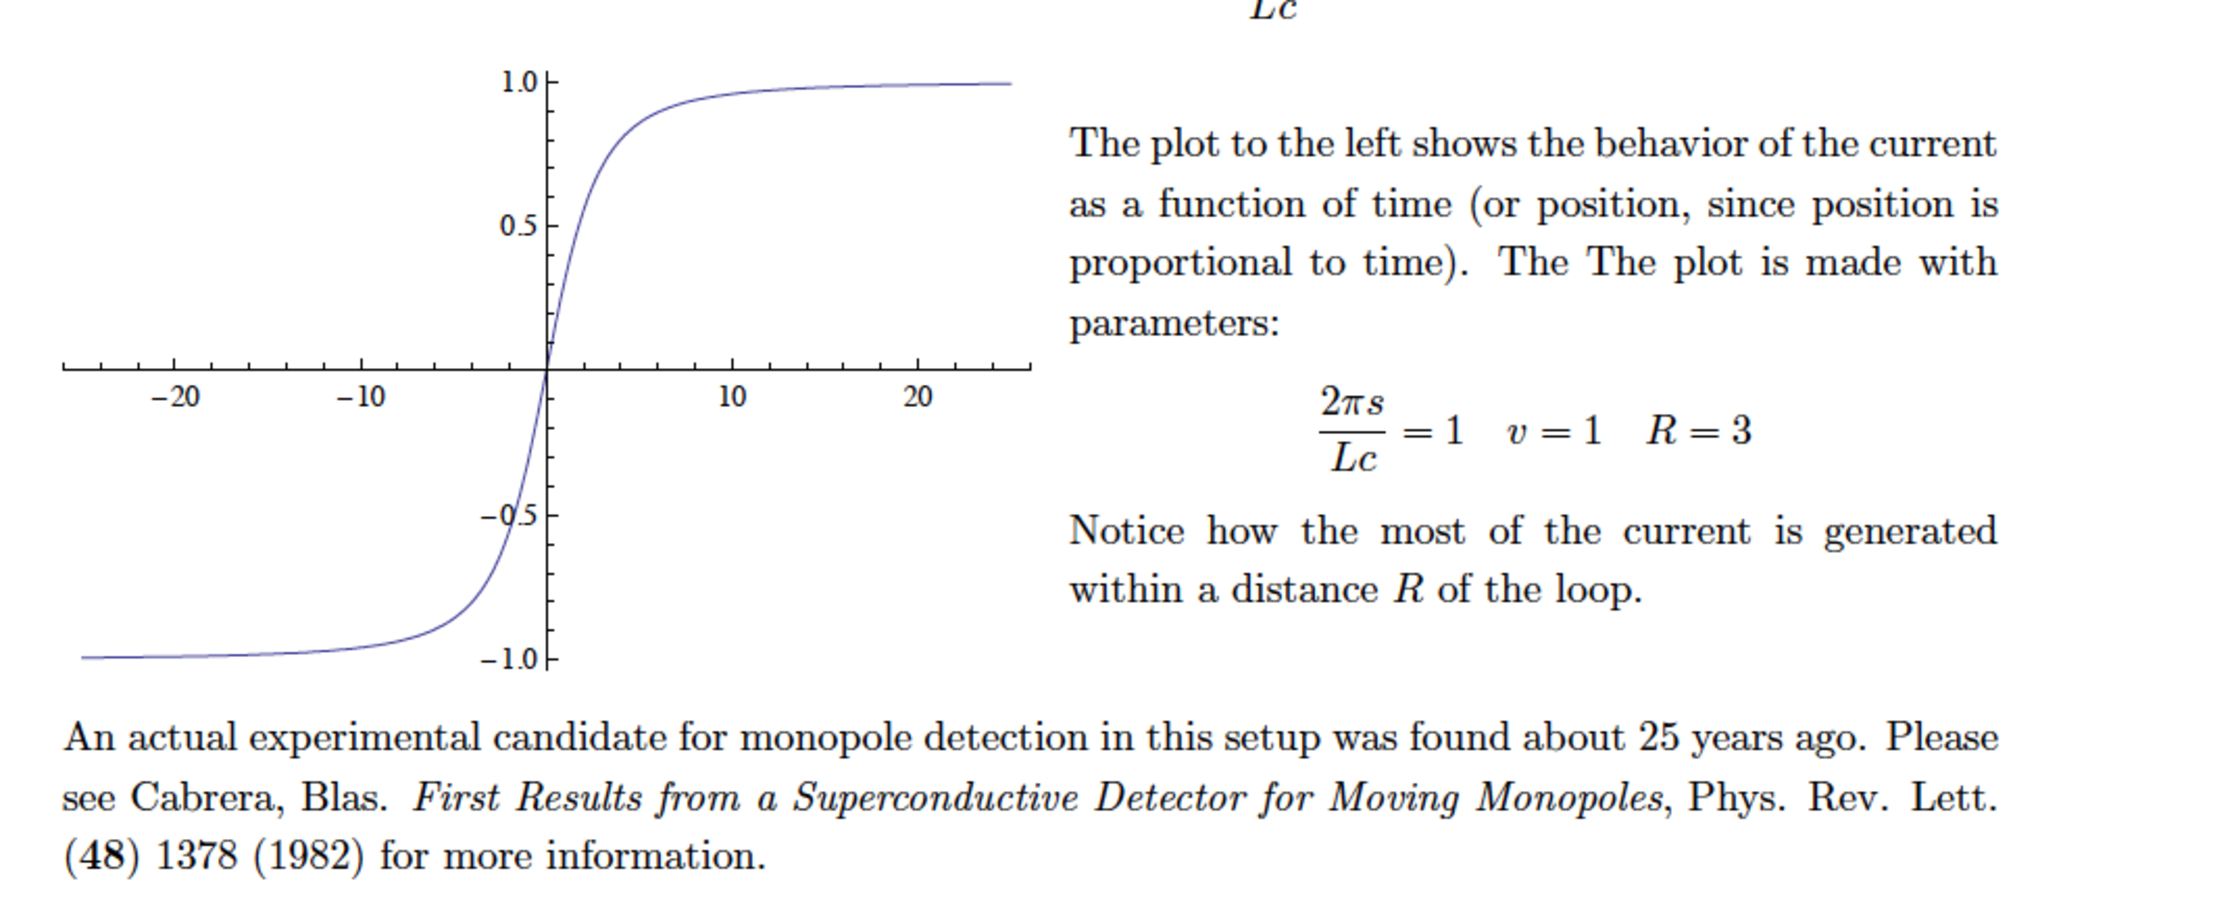
\includegraphics[width = 15cm]{monopole_sol_c}
    \caption{Magnetic monopole}
   \end{figure}

     \begin{figure}[H]
    \centering
    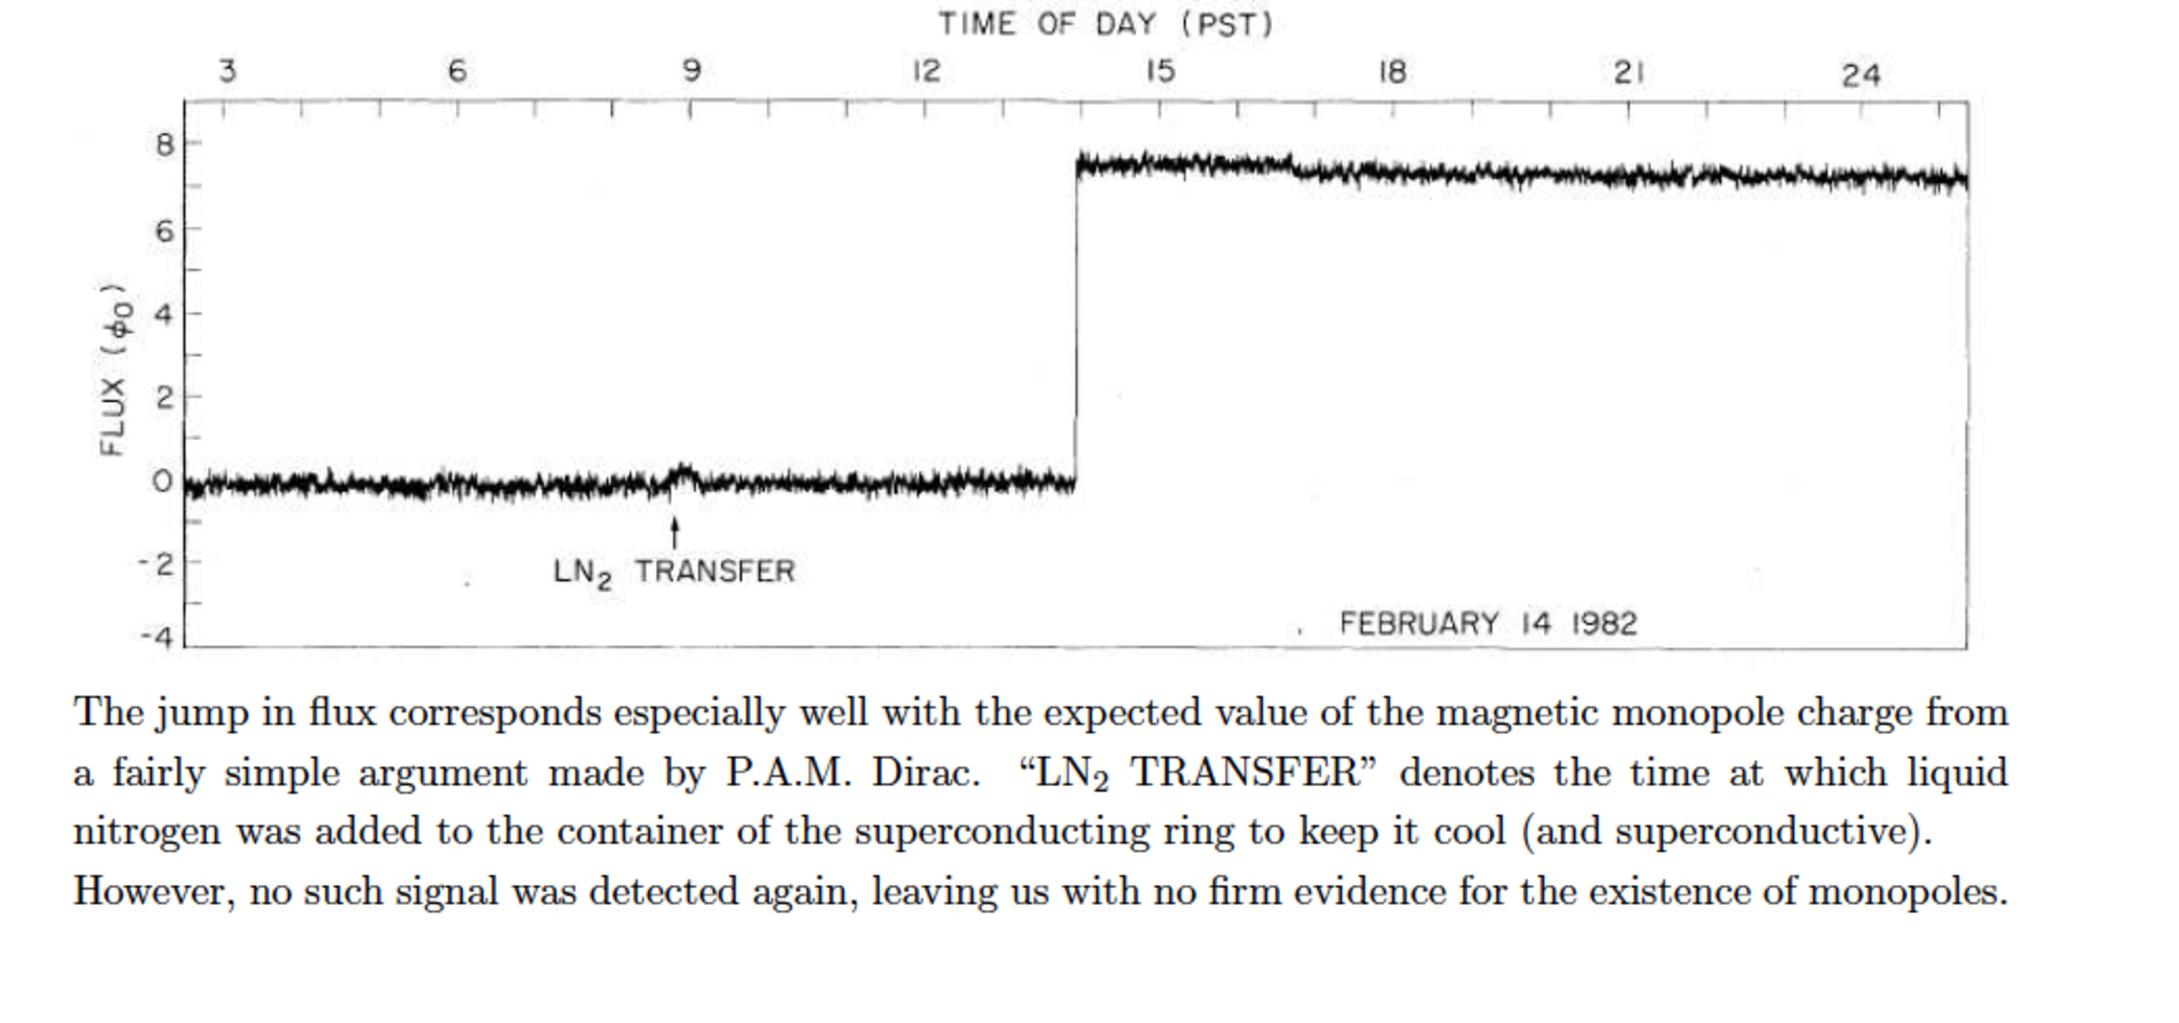
\includegraphics[width = 15cm]{monopole_sol_d}
    \caption{Magnetic monopole}
\end{figure}

\section{Problem \thesection: The Director's Challenge --- Extra credit!!!}
\subsection{Problem}
  Formulate an interesting problem that relates a topic from 8.022 to your
  intended major or any other topic about which you are passionate.  Give references
  to help future students to understand the context.  Try to give a solution.
  Any method --- theoretical, analytical, numerical, experimental --- is acceptable.
  If you can't give a full solution, outline partial solutions. Enjoy!
\end{document}
